% Options for packages loaded elsewhere
\PassOptionsToPackage{unicode}{hyperref}
\PassOptionsToPackage{hyphens}{url}
%
\documentclass[
]{article}
\usepackage{amsmath,amssymb}
\usepackage{lmodern}
\usepackage{iftex}
\ifPDFTeX
  \usepackage[T1]{fontenc}
  \usepackage[utf8]{inputenc}
  \usepackage{textcomp} % provide euro and other symbols
\else % if luatex or xetex
  \usepackage{unicode-math}
  \defaultfontfeatures{Scale=MatchLowercase}
  \defaultfontfeatures[\rmfamily]{Ligatures=TeX,Scale=1}
\fi
% Use upquote if available, for straight quotes in verbatim environments
\IfFileExists{upquote.sty}{\usepackage{upquote}}{}
\IfFileExists{microtype.sty}{% use microtype if available
  \usepackage[]{microtype}
  \UseMicrotypeSet[protrusion]{basicmath} % disable protrusion for tt fonts
}{}
\makeatletter
\@ifundefined{KOMAClassName}{% if non-KOMA class
  \IfFileExists{parskip.sty}{%
    \usepackage{parskip}
  }{% else
    \setlength{\parindent}{0pt}
    \setlength{\parskip}{6pt plus 2pt minus 1pt}}
}{% if KOMA class
  \KOMAoptions{parskip=half}}
\makeatother
\usepackage{xcolor}
\IfFileExists{xurl.sty}{\usepackage{xurl}}{} % add URL line breaks if available
\IfFileExists{bookmark.sty}{\usepackage{bookmark}}{\usepackage{hyperref}}
\hypersetup{
  pdftitle={Fixed and adaptive landmark sets for finite metric spaces},
  pdfauthor={Jason Cory Brunson; Yara Skaf},
  hidelinks,
  pdfcreator={LaTeX via pandoc}}
\urlstyle{same} % disable monospaced font for URLs
\setlength{\emergencystretch}{3em} % prevent overfull lines
\providecommand{\tightlist}{%
  \setlength{\itemsep}{0pt}\setlength{\parskip}{0pt}}
\setcounter{secnumdepth}{5}
\usepackage{format}
\ifLuaTeX
  \usepackage{selnolig}  % disable illegal ligatures
\fi

\title{Fixed and adaptive landmark sets for finite metric spaces}
\author{Jason Cory Brunson \and Yara Skaf}
\date{}

\begin{document}
\maketitle

\pagebreak

\hypertarget{introduction}{%
\section{Introduction}\label{introduction}}

Topological data analysis (TDA) is a maturing field in data science, at
the interface of statistics, computer science, and mathematics. Topology
is the discipline at the interface of geometry (the study of shape) and
analysis (the study of continuity) that focuses on geometric properties
that are preserved under continuous transformations. TDA consists in the
use of computational theories of continuity to investigate the shape or
structure of data. While TDA is most commonly associated with persistent
homology (PH) and mapper-like constructions, it can be understood to
generalize many conventional and even classical techniques, including
cluster analysis, network analysis, and nearest neighbors prediction.

Two frequent maneuvers in TDA are locality preservation and cardinality
reduction. \emph{Locality preservation} is the property of some
functions, such as projections or hashes, that nearby cases or points in
the domain have nearby images in the codomain. (Continuity, as defined
in analysis and topology, is a type of locality preservation.) This is
the defining property of many non-linear dimensionality reduction
techniques, including t-SNE and UMAP, but also an asymptotic property of
nearest neighbors prediction and the locally-sensitive hashing used in
its implementations. We use the term \emph{cardinality
reduction}\footnote{The term ``cardinality reduction'' takes different
  meanings in the data analysis literature, including the combining of
  different values of a categorical variable {[}@MicciBarreca2001;
  @Refaat2010{]} or of time series {[}@Hu2011{]} (also ``numerosity
  reduction'' {[}@Lin2007{]}). Our meaning is that of
  @ByczkowskaLipinska2017: an \(n\times p\) data table of \(n\) cases
  (rows) and \(p\) variables (columns) can be dimension-reduced to an
  \(n\times q\) table, where \(q<p\), or cardinality-reduced to an
  \(m\times p\) table, where \(m<n\). The most common cardinality
  reduction method is data reduction.}, in contrast to dimension
reduction, to describe techniques that produce more tractable or
comprehensible representations of complex data by reducing the number of
units of analysis rather than the number of variables or dimensions used
to represent them. For example, cardinality reduction describes cluster
analysis, which maps cases to clusters, and association network
analysis, which projects incidences or measurements to co-occurrence or
correlation relations.

More elaborate TDA techniques combine both maneuvers, often through the
use of covering methods, as with the approximation of PH through witness
complexes {[}@deSilva2004{]} or in the mapper construction
{[}@Singh2007{]}. Covering methods, in turn, can be enhanced by
strategic sampling from large data sets {[}@{]}, as can other
distance-based techniques like nearest neighbors. The maxmin sampling
procedure is often used for this purpose, as it is deterministic, is
computationally efficient, and generates more evenly distributed samples
than random selection. However, maxmin comes with its own limitations in
the analysis of data that vary greatly in density or have many
multiplicities. This is a frequent concern when sparse, heterogeneous,
and incomplete data are modeled as finite pseudometric spaces.

In this paper, we develop a sampling procedure complementary to maxmin,
based on the rankings of points by a distance or similarity measure
rather than on their raw values. In the remainder of this section, we
motivate the procedure, which we call lastfirst, as a counterpart to
maxmin obtained by adapting this procedure from the use of fixed-radius
balls to the use of fixed-cardinality neighborhoods. We work through an
extended example that illustrates some common patterns of clinical data
and models, how they cause problems for uses of maxmin landmark
selection, and how lastfirst selection addresses these problems. We then
formally describe the procedure and prove some of its basic properties
in Section\nbs\ref{sec:procedures}. This technical discussion is
accompanied by a small example in \(\Z\) that spotlights edge cases and
how they are handled, and it is followed by an example that extends the
method from 1 to 2 dimensions. In Section\nbs\ref{sec:implementation} we
report the results of benchmark tests and robustness checks of lastfirst
on simulated and empirical data sets. We describe some basic and novel
applications to real-world data in Section\nbs\ref{sec:experiments}.

\hypertarget{maxmin}{%
\subsection{Maxmin}\label{maxmin}}

The maxmin procedure is defined in
Section\nbs\ref{sec:maxmin}.\footnote{This procedure is distinct from
  many other uses of ``maxmin'' and related terms.} We designed the
lastfirst procedure to addresses an issue with maxmin that arises when,
due to the use of binary or categorical variables or to limits on
measurement resolution, a data set includes many duplicate or otherwise
indistinguishable cases. While these issues may be negligible when such
points are rare, they raise computational and interpretative concerns
when they are common.

Maxmin has often been used in TDA. @deSilva2004 propose witness
complexes, later generalized to alpha complexes {[}@{]}, for the rapid
approximation of PH: Given a point cloud, a set of landmark points and
their overlapping neighborhoods define a nerve, which stands in for the
Vietoris--Rips complex at each scale. They use maxmin as an alternative
to selecting landmark points uniformly at random. The procedure ensures
that the landmarks are locally separated and roughly evenly distributed.
Other uses include the selection of a sample of points from a
computationally intractable point cloud for the purpose of downstream
topological analysis, as when performing the mapper construction
{[}@Singh2007{]}; and the heuristic optimization of a fixed-radius ball
cover of a point cloud, in the sense of minimizing both the number of
balls and their shared radius {[}@Dlotko2019{]}. In addition to
approximating PH, maxmin was used in these cases to reduce the sizes of
simplicial complex models of point cloud data for the sake of
visualization and exploration.

\hypertarget{motivation}{%
\subsection{Motivation}\label{motivation}}

The ball covers mentioned above have been proposed as an alternative to
mapper {[}@Dlotko2019{]}, where they exchange discretion for
computational cost, and the mapper construction itself relies on a
crucial covering step that has received limited theoretical attention.
Conventionally, mappers rely on covers consisting either of overlapping
intervals (when the lens is one-dimensional) or of their cartesian
products (higher-dimensional). For this purpose, we propose that ball
covers, heuristically optimized using the maxmin procedure, have a
potential advantage over conventional covers, alongside a potential
disadvantage.

Conventionally, mappers use low-dimensional lens spaces \(\mathbb{R}^p\)
and one of two types of cover, based on overlapping intervals either of
fixed-length or at fixed quantiles {[}@; @Piekenbrock2020{]}. We think
of this length or quantile as the \emph{resolution} of the cover. When
\(m>1\), covers for \(Y\subset\mathbb{R}^m\) can be obtained as the
cartesian products of those of the coordinate projections of \(Y\)---so,
if \(\pi_1,\pi_2:\mathbb{R}^2\to\mathbb{R}\) are the coordinate
projections, then interval covers \(\{I_\alpha\}\) and \(\{J_\beta\}\)
of \(\pi_1(Y)\) and \(\pi_2(Y)\) give rise to the rectangle cover
\(\{I_\alpha \times J_\beta\}\) for \(Y\). While these cover types are
manageable in very few dimensions, the number of sets scales
geometrically with \(p\), holding the resolution fixed. Moreover,
eventually most of the resulting cover sets will contain no points of
\(X\), and additional calculations will be needed to restrict to the
non-empty sets. In contrast, a cover obtained by centering balls at a
subset of landmark points in \(Y\) will have greater up-front
computational cost but will be guaranteed to contain no empty sets, and
the number of sets required to capture the topology of \(Y\) will
increase only with the geometric and topological complexity of \(Y\),
not with \(p\). (We test this hypothesis in
Section\nbs\ref{sec:experiments}.)

Moreover, the maxmin cover requires not a coordinatization but only a
distance measure: the dissimilarity of cases \(x\) and \(y\) is captured
by their distance \(d(x,y)\), regardless of where \(x\) and \(y\) are
located in \(X\), and the neighborhoods \(B_r(x)\) and \(B_r(y)\) about
landmarks \(x\) and \(y\) play an equal role in the cover.\footnote{Is
  there a term for this property, e.g.~something being a ``universal
  constant''?} This means, however, that cover sets centered at
landmarks in sparse regions of \(X\) will be more numerous and of lower
cardinality than those centered in dense regions. While this assumption
is often made for convenience, it often does not hold in practice,
including in much of biomedicine.

This motivates us to produce a counterpart to the ball cover that we
call the \emph{neighborhood cover}, each set of which may have a
different radius but (roughly) the same cardinality. Especially in
analyses of medical and healthcare data, underlying variables can often
only be understood as ordinal, and high-dimensional data sets are
commonly analyzed using similarity measures rather than coordinate
embeddings. Furthermore, because measurements are coarse and often
missing, such data often contain indistinguishable entries---cases all
of whose measurements are equal and that are therefore represented as
multiple instances of the same point. All of these attributes violate
the assumptions of the ball cover approach and suggest the need for an
ordinal counterpart.

\hypertarget{illustration}{%
\subsection{Illustration}\label{illustration}}

Imagine an intensive care unit whose patients fall roughly into three
groups: a large, clinically homogeneous, low-risk majority; a smaller,
more heterogeneous, higher-risk group; and a minority of highly
distinctive patients who cannot be sorted into either group and are at
less predictable risk.

The top panel of Figure\nbs\ref{fig:icu-cover} depicts a simple model of
this situation in which each group is represented by a Gaussian
distribution. The shape approximates an empirical distribution of
standard risk scores observed for patients in the MIMIC-III database
(see Section\nbs\ref{sec:mimic}). (Imagine that probabilistic risk has
been logit-transformed, so that all real values are possible risk
estimates.) The points \(X\) along the abscissa are sampled randomly
from this distribution.

The bottom panel of Figure\nbs\ref{fig:icu-cover} shows how the maxmin
and lastfirst procedures generate sequences in \(X\) of four landmarks
each. Each procedure begins with a seed landmark \(\ell_0\) selected to
be reachable by minimum-radius balls (maxmin) or by minimum-cardinality
neighborhoods (lastfirst) from all other points in \(X\); see the
appendix for details. Whereas the maxmin landmarks are roughly
equally-spaced across the range of \(X\), the lastfirst landmarks lie at
roughly equal quantiles of \(X\). The lastfirst procedure will be
advantageous when subpopulations can be discriminated at different
resolutions and the ability to do so is limited primarily by sample
size.

\begin{figure}
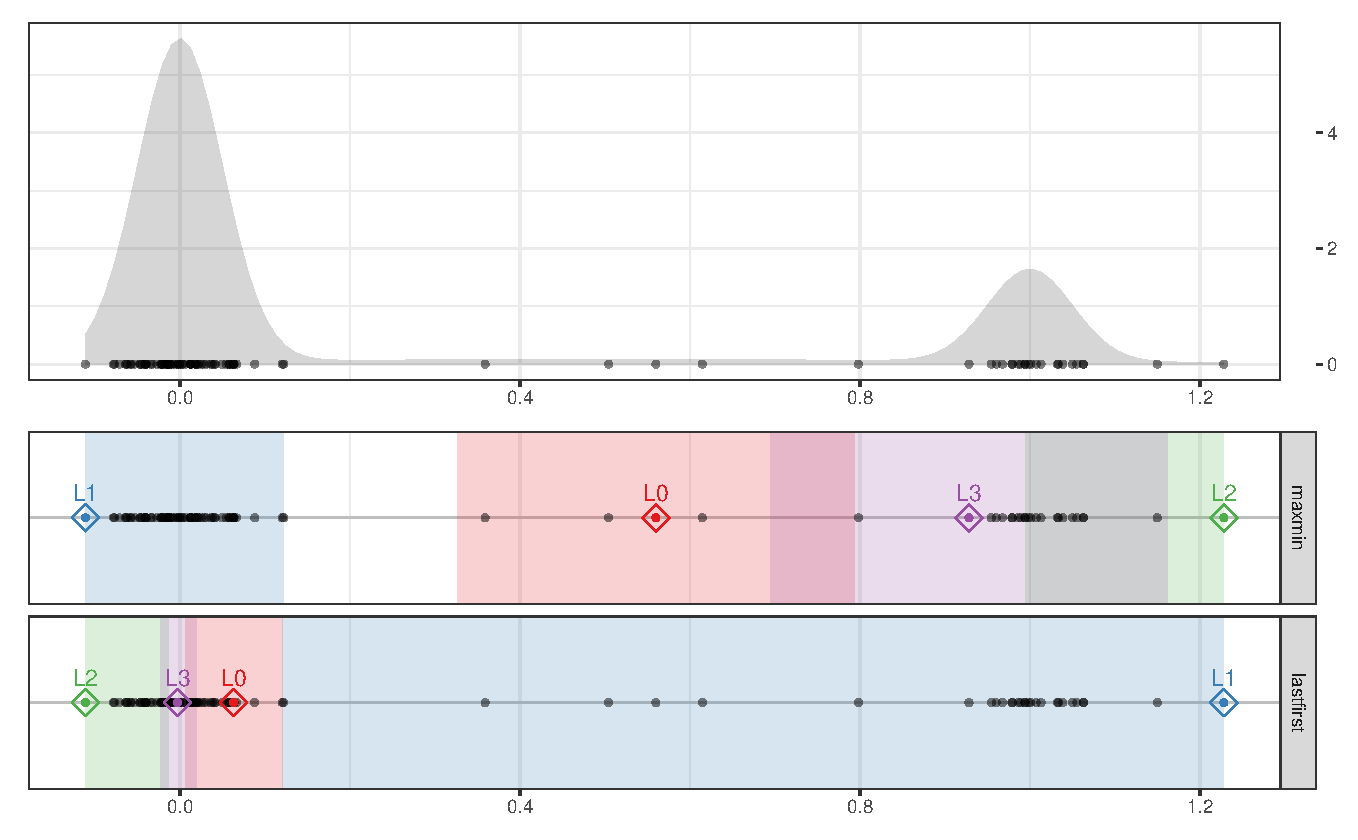
\includegraphics[width=\textwidth]{../figures/vardens-cover}
\caption{
Landmark samples from the imagined ICU sample and their associated covers using two selection procedures.
\label{fig:icu-cover}
}
\end{figure}

\hypertarget{procedures}{%
\section{Procedures}\label{procedures}}

\label{sec:procedures}

In this section we review the maxmin procedure and introduce the
lastfirst procedure as a complement to it.

\hypertarget{conventions}{%
\subsection{Conventions}\label{conventions}}

\((X, d_X)\) will refer to a finite pseudometric space with point set
\(X\) and pseudometric \(d_X:X\times X\to\R_{\geq 0}\), which by
definition satisfies all of the properties of a metric except that
\(d_X(x,y)=0\) implies \(x=y\). \((X,d_X)\) may be shortened to \(X\),
and \(d_X\) to \(d\), when clear from context. If \(x\neq y\) but
\(d(x,y)=0\) then \(x\) and \(y\) are said to be indistinguishable or
co-located. The cardinality of \(Y\subseteq X\) (counting
multiplicities) is denoted \(\abs{Y}\), the set of points co-located
with those in \(Y\) is denoted \(\cl{Y}\), and the set of equivalence
classes of \(Y\) under co-location is denoted \(\supp{Y}\). When
\(Y,Z\subseteq X\), let \(Y\wo Z\) denote the set difference
\(\{x \mid x \in Y \wedge x \notin Z\}\). Then \(Y \wo \cl{Z}\) is the
set of points in \(Y\) (with multiplicities) that are distinguishable
from all points in \(Z\). This means that, when defined,
\(\min_{y\in Y\wo \cl{Z},z\in Z}{d(y, z)}>0\).

We denote the diameter of \(Y\) as \(D(Y)=\max_{x,y\in Y}{d(x,y)}\), and
we write: \begin{align*}
d(Y,Z) &= \min_{y\in Y,z\in Z}{d(y,z)} & D(Y,Z) &= \max_{y\in Y,z\in Z}{d(y,z)} \\
d(x,Y) &= d(\{x\},Y)                   & D(x,Y) &= D(\{x\},Y) \\
\end{align*} If, for any \(x,y,z,w \in X\), \(d(x,y)=d(z,w)\) implies
\(\{x,y\}=\{z,w\}\)---that is, if no two pairs of points in \(X\) have
equal distance---then \(X\) is said to be in general position. We also
say that \(X\) is in \emph{locally general position} if, for any
\(x,y,z \in X\), \(d(x,y)=d(x,z)\) implies \(y=z\)---a weaker condition,
since there may exist \(w \in X\) for which \(d(x,y)=d(z,w)\) but
\(\{x,y\}\neq\{z,w\}\). Either condition implies that \(X\) is Hausdorff
(\(d(x,y)=0\implies x=y\)). \(f:X \to Y\) will denote a morphism of
pseudometric spaces, which we take to be a \(1\)-Lipschitz map
(\(d_X(x,y)\geq d_Y(f(x),f(y))\)).

Denote by \(\power{X}\) the power set of \(X\) and by \(\order{X}\) the
set of ordered, non-duplicative sequences from \(X\). We use the ball
notation \(B_{\eps}(x) \in \power(X)\) for the set of points less than
distance \(\eps\) from a point \(x\); that is,
\(B_{\eps}(x) = \{ y \mid d(x,y) < \eps \}\). We use an overline to also
include points exactly distance \(\eps\) from \(x\):
\(\cl{B_{\eps}}(x) = \{ y \mid d(x,y) \leq \eps \}\). (Every such ball
is both open and closed.) If \(\abs{\cl{B_\eps}(x)} \geq k\) and
\(\eps'<\eps \implies \abs{\cl{B_{\eps'}}(x)} < k\), then we call
\(N_k(x) = \cl{B_\eps}(x)\) the \(k\)-nearest neighborhood of \(x\).
When \(X\) is in locally general position, \(\abs{N_k(x)} = k\).

Throughout, let \(N=\abs{X}\). For convenience, we assume \(0\in\N\).
For \(a,b \in \N\) with \(a<b\), we use \([a,b]\) to denote the
arithmetic sequence \((a,a+1,\ldots,b)\). For \(a,b \in \N\), we use
\(a^b\) to denote the sequence \((a,\ldots,a)\) of length \(b\).

\hypertarget{maxmin-procedure}{%
\subsection{Maxmin procedure}\label{maxmin-procedure}}

\label{sec:maxmin}

\begin{definition}[maxmin]\label{def:maxmin}
Given $(X,d)$ and $Y\subset X$, define the \emph{maxmin set}
$$\maxmin(Y;X) = \maxmin(Y) = \{ x \in X \wo \cl{Y} \mid d(x,Y) = \max_{y\in X\wo \cl{Y}}{d(y,Y)} \}$$
consisting of \emph{maxmin points}.
\end{definition}

Note that \(\maxmin(Y)\) is nonempty when
\(X \wo \cl{Y} \neq \varnothing\) and that \(\maxmin(Y)\) has
cardinality \(1\) when \(X\) is in locally general position.

\begin{algorithm}
\caption{Select a maxmin landmark set.}
\label{alg:maxmin}
\begin{algorithmic}[1]
\REQUIRE finite metric space $(X,d)$
\REQUIRE at least one parameter $\eps\geq 0$ or $n\in\N$
\REQUIRE seed point $\ell_0 \in X$
\IF{only $\eps$ is given}
    \STATE $n \leftarrow 1$
\ENDIF
\IF{only $n$ is given}
    \STATE $\eps \leftarrow \infty$
\ENDIF
\STATE $L \leftarrow \varnothing$
\STATE $i \leftarrow 0$
\REPEAT
    \STATE $L \leftarrow L\cup\{\ell_i\}$
    \STATE $i \leftarrow i+1$
    \STATE $\ell_i \in \maxmin(L)$
    \STATE $d_{\operatorname{max}} \leftarrow d(\ell_i,L)$
\UNTIL $d_{\operatorname{max}} < \eps$ and $\abs{L} \geq n$
\RETURN maxmin landmark set $L$
\end{algorithmic}
\end{algorithm}

The \emph{maxmin procedure} for generating a landmark set
\(L\subseteq X\) proceeds as follows (see
Algorithm\nbs\ref{alg:maxmin}). Each step receives a proper subset
\(L\subset X\) and returns a point \(x\in X\wo \cl{L}\).

First, choose a number \(n\leq\uniq{X}\) of landmark points to generate
or a radius \(\eps\geq 0\) for which to require that the balls
\(\{ \cl{B_{\eps}}(\ell) : \ell \in L \}\) cover \(X\). Choose a first
landmark point \(\ell_0\in X\). Inductively over \(i\in\N\), if ever
\(i\geq n\) or \(d(L,X\wo \cl{L})\leq\eps\), then stop. Otherwise, when
\(L=\{\ell_0,\ldots,\ell_{i-1}\}\), choose \(\ell_i\in\maxmin(L)\),
according to a preferred procedure \(\sigma\) (see the Appendix). If a
fixed number \(n\) of landmarks was prescribed, then set
\(\eps=\eps(n)=d(L,X\wo \cl{L})\); if \(\eps\) was prescribed and
\(\sigma\) is understood, then set \(n=n(\eps)=\abs{L}\). Write
\(\mathcal{B}_\eps(\ell_0)=\{\cl{B_{\eps}(\ell_i)}\}_{i=0}^{n}\) for the
resulting \emph{landmark cover of $X$}.

We will write the elements of landmark sets
\(L=\{\ell_0,\ldots,\ell_{n-1}\}\) in the order in which they were
generated. Note that, if \(n=\uniq{X}\) or \(\eps=0\), then
\(\cl{L}=X\). When the procedure stops,
\(X=\bigcup_{i=0}^{n-1}{\cl{B_{\eps}}(\ell_i)}\). This cover is not, in
general, a minimal cover, but it is a minimal landmark cover in the
sense that the removal of \(\cl{B_\eps}(\ell_{n-1})\) and any decrease
in \(\eps\) will yield a collection of sets that fail to cover \(X\). A
``thickened'' cover can be obtained by pre-specifying both \(n\) and
\(\eps\) in such a way that \(n \geq n(\eps)\) and
\(\eps \geq \eps(n)\). In Section\nbs\ref{sec:implementation}, we
describe two adaptive parameters implemented in our software package
that make these choices easier.

\hypertarget{lastfirst-procedure}{%
\subsection{Lastfirst procedure}\label{lastfirst-procedure}}

Let us redefine the maxmin procedure in terms of balls rather than of
distances:

\begin{proposition}[maxmin in terms of balls]\label{prop:maxmin}
    Given $(X,d)$ and $Y \subset X$, write $B_\eps(Y) = \bigcup_{y \in Y}{B_\eps(y)}$ and similarly for closed balls, then let
    $$\Eps(Y,X) = \min\{ \eps \mid \cl{B_\eps}(Y) = X \}$$
    Then
    $$\maxmin(Y;X,d) = X \wo B_{\Epsilon(Y,X)}(Y)$$
\end{proposition}

The lastfirst procedure is defined analogously to the maxmin procedure,
substituting nearest neighborhoods, parameterized by their cardinality
\(k\), for balls, parameterized by their radius \(\eps\). Membership in
nearest neighborhoods is not a symmetric relation: It may be that
\(y \in N_k(x)\) while \(x \notin N_k(y)\). We therefore introduce a
companion concept that reverses this relationship:

\begin{definition}[$k$-neighborhoods]
    For $x \in X$, define the \emph{$k$-out-neighborhoods} $N^+_k$ and \emph{$k$-in-neighborhoods} $N^-_k$ of $x$ as the sets
    \begin{align*}
        N^+_k(x) &= \{ y\in X \mid y \in N_k(x) = N_k(x) \} \\
        N^-_k(x) &= \{ y\in X \mid x \in N_k(y) \}
    \end{align*}
    Given a subset $Y \subseteq X$, we also define
    \begin{align*}
        N^+_k(x,Y) &= Y \cap N^+_k(x) \\
        N^-_k(x,Y) &= Y \cap N^-_k(x)
    \end{align*}
\end{definition}

Note that
\([\{x\}] = N^\pm_0(x) \subseteq \cdots \subseteq N^\pm_{N-1}(x) = X\).
The \(k\)-out-neighborhoods of \(x\) are the \(k\)-nearest neighbors of
\(x\), i.e.~the sets of points in \(X\) that have out-rank at most \(k\)
from \(x\). The \(k\)-in-neighborhoods of \(x\) are the sets of points
in \(X\) from which \(x\) has out-rank at most \(k\).

\begin{example}\label{ex:rank-neighborhoods}
Consider the same $X$ as in Example\nbs\ref{ex:relative-rank}. Compute $N_k^+$ and $N_k^-$ for $a$ and $c$, using $k = 3$:
\begin{align*}
    N_3^+ (a) &= \{a, b, c, d\} &
    N_3^+ (c) &= \{b, c, d\} \\
    \\
    N_3^- (a) &= \{a, b\} &
    N_3^- (c) &= \{a, b, c, d\}
\end{align*}
\end{example}

\begin{remark}
If $\abs{N^\pm_k(x)} = n_k$, then $\abs{N^\pm_k(x,X\wo\{x\})} = n_k - 1$.
\end{remark}

\hypertarget{rank-sequences-and-landmark-selection}{%
\subsubsection{Rank sequences and landmark
selection}\label{rank-sequences-and-landmark-selection}}

Maxmin is a heuristic, iterative procedure used to select a
well-dispersed subset of points from \(X\), where dispersion is
understood in terms of the interpoint distances of this subset. At each
step, landmarks \(L = \{\ell_0, \ldots, \ell_{i-1}\}\) having been
selected, the next point \(\ell_i\) is selected to maximize its minimum
distance \(d(\ell_j,\ell_i)\) from the \(\ell_j\), \(0 \leq j < 1\).
Equivalently, \(\ell_i \in X \wo L\) is selected so that the minimum
radius \(\eps\) required for
\(\ell_i \in \bigcup_{j=0}^{i-1}{\cl{B_\eps}(\ell_j)}\) is maximized.
This is a useful heuristic for constructing a ball cover
\(\mathcal{B} = \{\cl{B_\eps}(\ell_j) \mid 0 \leq j < n\}\) centered at
a highly mutually distant set of landmarks.

We desire to construct a neighborhood cover
\(\mathcal{N} = \{N^+_k(\ell_j) \mid 0 \leq j < n\}\) whose centers are
analogously dispersed. Suppose \(\ell_i\) is selected so that the
minimum \(k\) required for
\(\ell_i \in \bigcup_{j=0}^{i-1}{N_k(\ell_j)}\) is maximized. This is
equivalent to maximizing the minimum out-rank \(q(\ell_j,\ell_i)\) of
\(\ell_i\) from any \(\ell_j\). Switching perspective from out- to in-
and reversing the roles of \(L\) and \(\ell_i\), we want
\(N^-_k(\ell_i,L)=0\) for the latest (largest) \(k\) possible, say
\(k^-_0\). When indistinguishable points abound, this may still not
uniquely determine \(\ell_i\), so we may extend the principle: Among
those \(\ell\in X\wo \cl{L}\) for which \(N^-_{k^-_0}(\ell_i,L)=0\),
choose \(\ell_i\) for which \(N^-_{k}(\ell_i,L) \leq 1\) for the latest
\(k\) possible, say \(k^-_1 \geq k^-_0\). (It is possible that
\(k^-_1 = k^-_0\), in which case no \(N^-_k(\ell_i,L) = 1\).) Continue
this process until only one candidate \(\ell\) remains (up to
multiplicity), or until \(N^-_{k}(\ell,L)=\abs{L}\), in which case all
remaining candidates may be considered equivalent.\footnote{Break this
  into a separate paragraph that analogizes \(\sigma\) from the maxmin
  discussion.} Example\nbs\ref{ex:rank-sequence} illustrates these
computations.

\begin{example}\label{ex:rank-sequence}
Continuing Example\nbs\ref{ex:rank-neighborhoods}, we can compute the other $N_\bullet^+$ and $N_\bullet^-$ for $a$ and $c$:
\begin{align*}
    N_\bullet^+ (a) &= (\abs{N^+_0(a)}, \abs{N^+_1(a)}, \abs{N^+_2(a)}, \abs{N^+_3(a)}) &
    N_\bullet^+ (c) &= (\abs{N^+_0(c)}, \abs{N^+_1(c)}, \abs{N^+_2(c)}, \abs{N^+_3(c)}) \\
    &= (\abs{\{a\}}, \abs{\{a, b\}}, \abs{\{a, b, c, d\}}, \abs{\{a, b, c, d\}}) &
    &= (\abs{\{c, d\}}, \abs{\{c, d\}}, \abs{\{b, c, d\}}, \abs{\{a, b, c, d\}}) \\
    &= (1, 2, 4, 4) &
    &= (2, 2, 3, 4) \\
    \\
    N_\bullet^- (a) &= (\abs{N^-_0(a)}, \abs{N^-_1(a)}, \abs{N^-_2(a)}, \abs{N^-_3(a)}) &
    N_\bullet^- (c) &= (\abs{N^-_0(c)}, \abs{N^-_1(c)}, \abs{N^-_2(c)}, \abs{N^-_3(c)}) \\
    &= (\abs{\{a\}}, \abs{\{a, b\}}, \abs{\{a, b\}}, \abs{\{a, b, c, d\}}) &
    &= (\abs{\{c, d\}}, \abs{\{c, d\}}, \abs{\{a, b, c, d\}}, \abs{\{a, b, c, d\}}) \\
    &= (1, 2, 2, 4) &
    &= (2, 2, 4, 4)
\end{align*}
\end{example}

\begin{definition}[total orders on rank sequences]
    Let $a_n = (a_1,\ldots,a_M),b_n = (b_1,\ldots,b_M)\in\N^M$.
    Then $a_n < b_n$ in the reverse lexicographic (revlex) order if $\exists i : a_i > b_i \wedge (\forall j<i : a_j = b_j)$.
\end{definition}

Impose the revlex order on the \(N_\bullet^+\) and \(N_\bullet^-\) to
emphasize the sizes of smaller neighborhoods. Sequences with more large
values indicate points with lower out-ranks to or from more other
points.

We now define counterparts to the minmax and maxmin procedures to be
used with these totally ordered sequences.

\begin{definition}[lastfirst, in terms of neighborhoods]
    Given $(X,d)$ and $Y \subset X$, write $N_k(Y) = \bigcup_{y \in Y}{N_k(y)}$, then let
    $$K(Y,X) = \min\{ k \mid N_k(Y) = X \}$$
    Then define the \emph{lastfirst set}
    $$\lf(Y;X,d) = \lf(Y) = X \wo N_{K(Y,X) - 1}(Y)$$
    consisting of \emph{lastfirst points}.
\end{definition}

\begin{example}
    Return again to $X=\{a,b,c,d\}$ from Example\nbs\ref{ex:relative-rank}. We calculate an exhaustive lastfirst landmark set, seeded with a point of minimal out-rank sequence:
    \begin{enumerate}
        \item We have
        \begin{align*}
            N_\bullet^+(a,\{b,c,d\}) &= (0,1,3,3) &
            N_\bullet^+(b,\{a,c,d\}) &= (0,1,3,3) \\
            N_\bullet^+(c,\{a,b,d\}) &= (1,1,2,3) &
            N_\bullet^+(d,\{a,b,c\}) &= (1,1,2,3)
        \end{align*}
        Under the revlex order, $\argmin_{x\in X}{N_\bullet^+(x,X \wo \cl{\{x\}})}=\{c,d\}$, and we arbitrarily select $\ell_0=c$ and $L=\{c\}$.
        \item For $x \in X \wo \cl{L}$ we now have
        \begin{align*}
            N_\bullet^-(a,\{c\}) &= (0,0,0,1) &
            N_\bullet^-(b,\{c\}) &= (0,0,1,1)
        \end{align*}
        Under the revlex order, $\argmax_{x\in X \wo \cl{\{c\}}}{N_\bullet^-(x,\{c\})}=\{a\}$; we select $\ell_1=a$, so that now $L=\{c,a\}$.
        \item Only one point remains in $X\wo \cl{L}=\{b\}$, so the exhaustive landmark set is $\{c,a,b\}$.
    \end{enumerate}
\end{example}

We defer algorithms and proofs to the Appendix, where we rely on
additional technical definitions. The results apply to a more general
conception of ``relative rank'' (our term), one of which is induced by
the pseudometric on any finite pseudometric space but which need only
satisfy the condition that a point is no nearer any other point than
itself.

\hypertarget{illustration-1}{%
\subsubsection{Illustration}\label{illustration-1}}

Consider the ``necklace'' data set adapted from {[}@{]}. The points are
sampled in the plane from a large, low-density circular region (the
``string'') and from several smaller, higher-density circular regions
(the ``beads'') evenly spaced along the string. Only a method of
detecting topology that is adaptive to the different scales of the
string and of the beads will recover both the large feature and the
smaller features of dimension 1. We use small landmark samples to
illustrate the differences between the maxmin and lastfirst selection
procedures, \textbf{and we compute the nerves of the covers obtained
from larger samples to test their ability to detect homology at multiple
scales}.

\begin{figure}
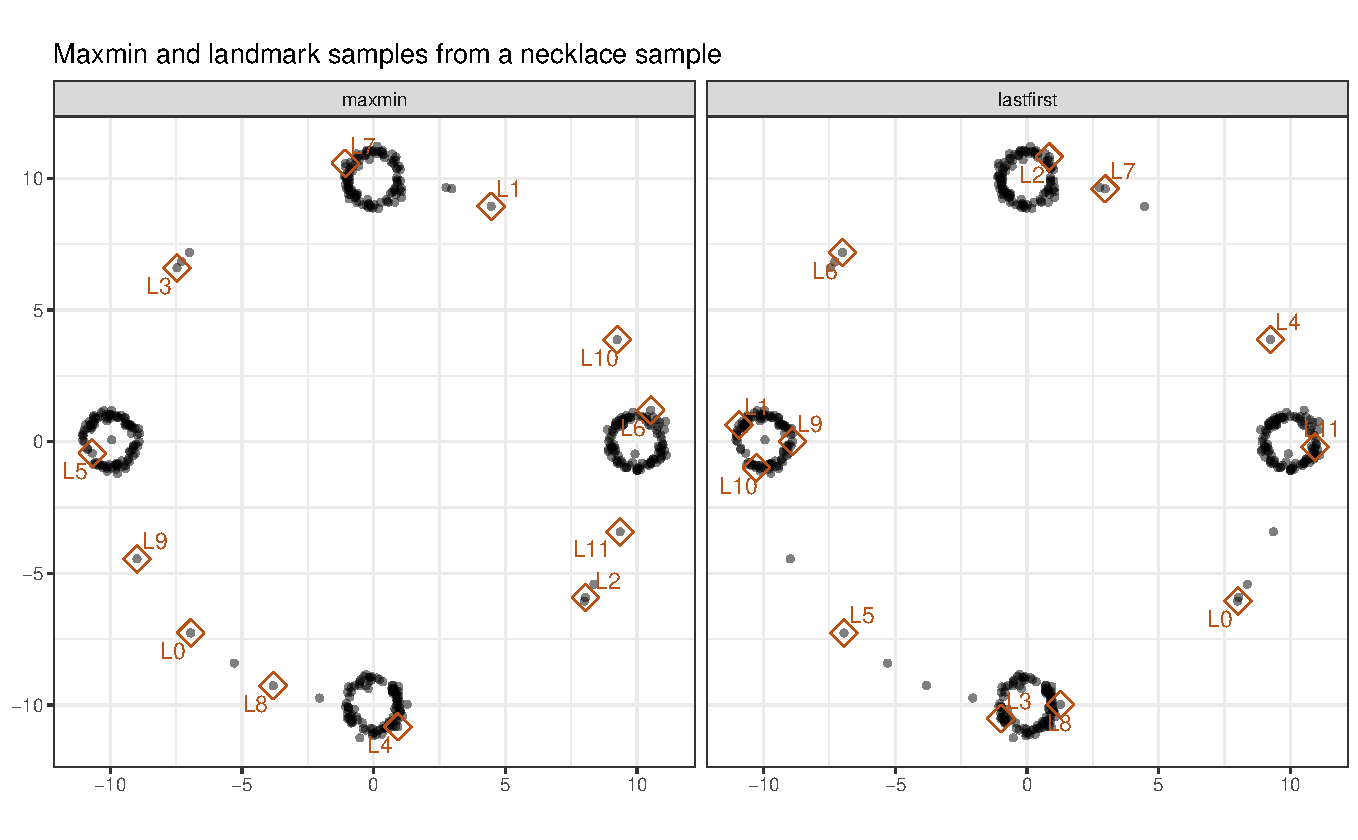
\includegraphics[width=\textwidth]{../figures/necklace-landmarks}
\caption{
Landmark samples of size 12 from a necklace data set using two selection procedures.
\label{fig:necklace}
}
\end{figure}

\hypertarget{implementation}{%
\section{Implementation}\label{implementation}}

\label{sec:implementation}

We have implemented the lastfirst procedure, together with maxmin, in
the R package landmark {[}@Brunson2021a{]}. Each procedure is
implemented for Euclidean distances in C++ using Rcpp
{[}@Eddelbuettel2011{]} and for many other distance metrics and
similarity measures in R using the proxy package {[}@Meyer2021{]}. For
relative rank--based procedures, the user can choose any tie-handling
rule. The landmark-generating procedures return the indices of the
selected landmarks, optionally together with the sets of indices of the
points in the cover set centered at each landmark. In addition to the
number of landmarks \(n\) and either the radius \(\eps\) of the balls or
the cardinality \(k\) of the neighborhoods, the user may also specify
additive and multiplicative extension factors for \(n\) and for \(\eps\)
or \(k\). These will produce additional landmarks (\(n\)) and larger
cover sets (\(\eps\) or \(k\)) with increased overlaps, in order to
construct more redundant covers.

\hypertarget{validation}{%
\subsection{Validation}\label{validation}}

We validated the firstlast and lastfirst procedures against several
small example data sets, including that of
Example\nbs\ref{ex:relative-rank}. We also validated the C++ and R
implementations against each other on several larger data sets,
including as part of the benchmark tests reported in the next section.
We invite readers to experiment with new cases and to request or
contribute additional features.

\hypertarget{benchmark-tests}{%
\subsection{Benchmark tests}\label{benchmark-tests}}

We benchmarked the C++ and R implementations on three data sets: uniform
samples from the unit circle \(\Sph^1\subset\R^2\) convoluted with
Gaussian noise, samples with duplication from the integer lattice
\([0,23]\times[0,11]\) using the probability mass function
\(p(a,b) \propto 2^{-ab}\), and patients recorded at each critical care
unit in MIMIC-III using RT-transformed data and cosine similarity
(Section\nbs\ref{sec:data}). We conducted benchmarks using the bench
package {[}@Hester2020{]} on the University of Florida high-performance
cluster HiPerGator.

\begin{figure}
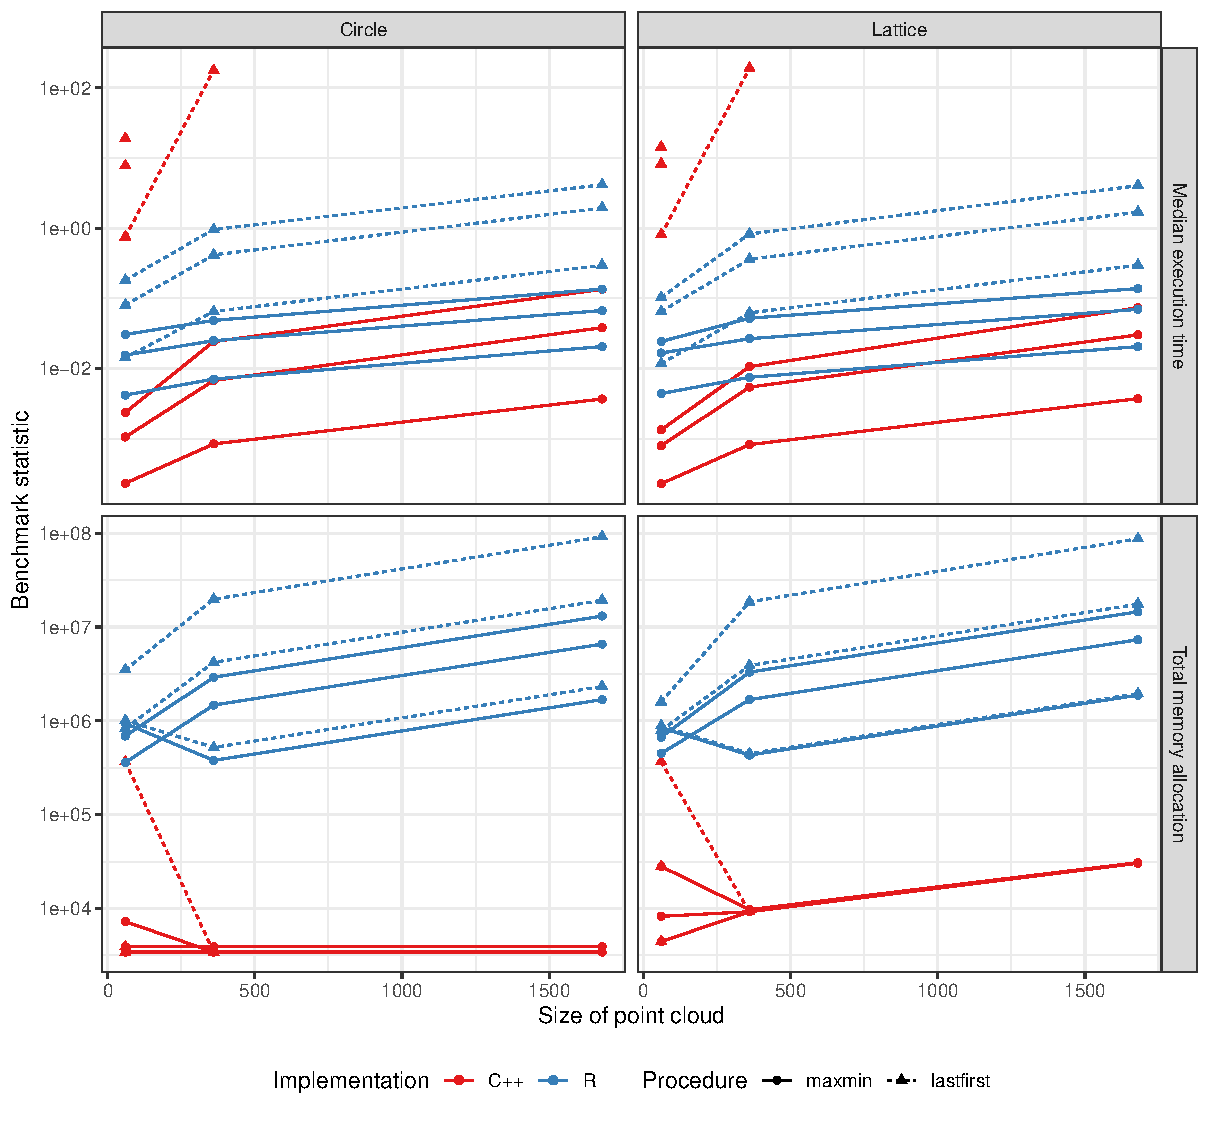
\includegraphics[width=.6666667\textwidth]{../figures/benchmark-circle-lattice}
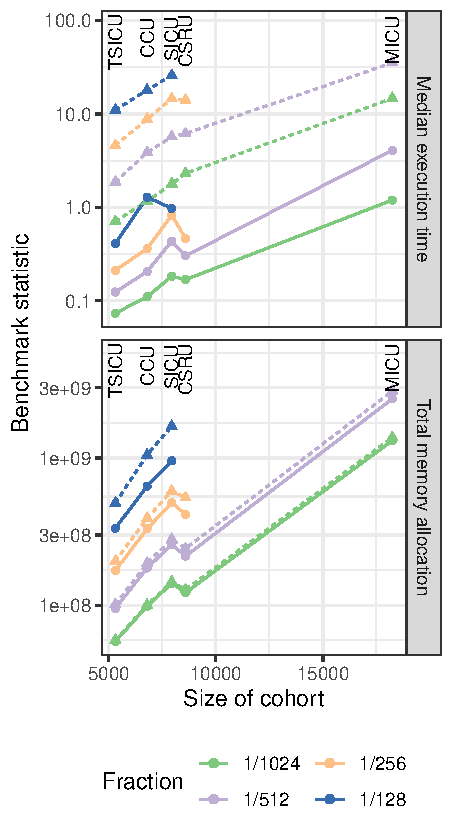
\includegraphics[width=.3333333\textwidth]{../figures/benchmark-mimic}
\caption{
Benchmark results for computing landmarks on two families of artificial data (circle and lattice) and one collection of empirical data (RT-similarity space of critical care units in MIMIC-III). Some points are missing because benchmark tests did not complete within 1 hour.
\label{fig:benchmark}
}
\end{figure}

Benchmark results are reported in Figure\nbs\ref{fig:benchmark}. The R
implementation of maxmin used orders of magnitude more memory and took
slightly longer. They appeared to scale slightly better in terms of time
and slightly worse in terms of memory. The additional calculations
required for the lastfirst procedure increase runtimes by a median
factor of 2.5 in our R implementations. The C++ implementation of
lastfirst is based on combinatorial definitions and not optimized for
speed, and as a result takes much longer---a median factor of almost
2000 relative to maxmin in C++---and failed to complete in many of our
tests.

\hypertarget{experiments}{%
\section{Experiments}\label{experiments}}

\label{sec:experiments}

\hypertarget{empirical-data}{%
\subsection{Empirical data}\label{empirical-data}}

\label{sec:data}

\hypertarget{mimic-iii}{%
\subsubsection{MIMIC-III}\label{mimic-iii}}

\label{sec:mimic}

The open-access critical care database MIMIC-III (``Medical Information
Mart for Intensive Care''), derived from the administrative and clinical
records for 58,976 admissions of 46,520 patients over 12 years and
maintained by the MIT Laboratory for Computational Physiology and
collaborating groups, has been widely used for education and research
{[}@Goldberger2000; @Johnson2016{]}. For our analyses we included data
for patients admitted to five care units: coronary care (CCU), cardiac
surgery recovery (CSRU), medical intensive care (MICU), surgical
intensive care (SICU), and trauma/surgical intensive care
(TSICU).\footnote{\url{https://mimic.physionet.org/mimictables/transfers/}}
For each patient admission, we extracted the set of ICD-9/10 codes from
the patient's record and several categorical demographic variables: age
group (18--29, decades 30--39 through 70--79, and 80+), recorded gender
(M or F), stated ethnicity (41 values),\footnote{White, Black/African
  American, Unknown/Not Specified, Hispanic or Latino, Other, Unable to
  Obtain, Asian, Patient Declined to Answer, Asian -- Chinese, Hispanic
  Latino --~Puerto Rican, Black/Cape Verdean, White -- Russian, Multi
  Race Ethnicity, Black/Haitian, Hispanic/Latino --~Dominican, White
  --~Other European, Asian -- Asian Indian, Portuguese, White
  --~Brazilian, Asian --~Vietnamese, Black/African, Middle Eastern,
  Hispanic/Latino --~Guatemalan, Hispanic/Latino -- Cuban, Asian --
  Filipino, White --~Eastern European, American Indian/Alaska Native,
  Hispanic/Latino --~Salvadoran, Asian -- Cambodian, Native Hawaiian or
  Other Pacific Islander, Asian -- Korean, Asian -- Other,
  Hispanic/Latino --~Mexican, Hispanic/Latino --~Central American
  (Other), Hispanic/Latino --~Colombian, Caribbean Island, South
  American, Asian -- Japanese, Hispanic/Latino -- Honduran, Asian --
  Thai, American Indian/Alaska Native Federally Recognized Tribe} stated
religion,\footnote{Catholic, unspecified/unobtainable/missing,
  Protestant Quaker, Jewish, other, Episcopalian, Greek Orthodox,
  Christian Scientist, Buddhist, Muslim, Jehovah's Witness,
  Unitarian-Universalist, 7th Day Adventist, Hindu, Romanian Eastern
  Orthodox, Baptist, Hebrew, Methodist, Lutheran} marital
status\footnote{married, single, widowed, divorced, unknown/missing,
  separated, life partner}, and type of medical insurance\footnote{Medicare,
  private, Medicaid, povernment, self pay}. Following @Zhong2020, we
transformed these \emph{relational-transaction (RT)} data into a binary
case-by-variable matrix \(X \in \B^{n \times p}\) suitable for the
cosine similarity measure, which was converted to a distance measure by
subtraction from 1. Because cosine similarity is monotonically related
to the angle metric, our topological results will be the same up to this
rescaling, so for simplicity we use cosine similarity in our
experiments.

\hypertarget{mexican-department-of-health}{%
\subsubsection{Mexican Department of
Health}\label{mexican-department-of-health}}

The Mexican Department of Health (MXDH) has released official
open-access data containing an assortment of patient-level clinical
variables related to COVID-19 infection and outcomes. These data have
been compiled into a database and made freely available on
Kaggle\footnote{\url{https://www.kaggle.com/lalish99/covid19-mx}}, a
collaborative data science platform. The data we obtained includes
information regarding over 724,000 patients confirmed to be
COVID-positive via diagnostic laboratory testing. Two main types of
information are present for each patient: (1) dates, and (2) categorical
or binary variables. The former are dates associated with key moments in
the clinical course of infection such as symptom onset, admission to a
healthcare institution, and death (if applicable). The categorical and
binary fields encode clinical factors likely to be associated with
COVID-19 infection, severity, or outcome. These variables include
information such as sex, state of patient residence, and intubation
status, as well as binary fields encoding the presence or absence of a
wide variety of comorbidities such as asthma, hypertension,
cardiovascular disease. (For a full description of each field included
in the data set, see Kaggle.*) Though these variables are categorical
rather than continuous/numeric, there are sufficiently many of them
(\(\approx 50\)) to potentially distinguish between many patient
phenotypes. Further, this data set is very complete in that every
patient is required to contain a valid value for every field, which
minimizes concerns around missing data.

\hypertarget{covers-and-nerves}{%
\subsection{Covers and nerves}\label{covers-and-nerves}}

Cardinality reduction techniques can be used to model a large number of
cases represented by a large number of variables as a smaller number of
clusters with similarity or overlap relations among them. The
deterministic maxmin and lastfirst procedures provide clusters (cover
sets) defined by proximity to the landmark cases and relations defined
by their overlap. The clusters obtained by these procedures occupy a
middle ground between the regular intervals or quantiles commonly used
to cover samples from Euclidean space and the emergent clusters obtained
heuristically by penalizing between-cluster similarity and rewarding
within-cluster similarity. The maxmin procedure produces cover sets of
(roughly) fixed radius, analogous to overlapping intervals of fixed
length, while the lastfirst procedure produces cover sets of fixed size,
analogous to the quantiles of an adaptive cover. This makes them natural
solutions to the task of covering an arbitrary finite metric space that
may or may not contain important geometric or topological structure
{[}@Singh2007{]}.

As a practical test of this potential, we loosely followed the approach
of @Dlotko2019 to construct covers and their nerves for each care unit
of MIMIC-III, using maxmin and lastfirst. We varied the number of
landmarks (6, 12, 24, 36, 48, 60, 120) and the multiplicative extension
of the cover sets' sizes (0, .1, .2). We evaluated the procedures in
three ways:

\begin{itemize}
\tightlist
\item
  \textbf{Clustering quality:} Both procedures yield \emph{fuzzy}
  clusters---that is to say, clusters that allow for some overlap. While
  clustering quality measures might be useful, most, including almost
  all that have been proposed for fuzzy clusterings, rely on
  coordinate-wise calculations, specifically data and cluster centroids
  {[}@Bouguessa2006; @Wang2007; @Falasconi2010{]}. To our knowledge, the
  sole exception to have appeared in a comprehensive comparison of such
  measures is the \emph{modified partition coefficient} {[}@Dave1996{]},
  defined as
  \[\operatorname{MPC}=1-\frac{k}{k-1}(1-\frac{1}{n}\sum_{i=1}^{n}{\sum_{j=1}^{k}{{u_{ij}}^2}})\]
  where \(U=(u_{ij})\) is the \(n\times k\) fuzzy partition matrix:
  \(u_{ij}\) encodes the extent of membership of point \(x_i\) in
  cluster \(c_j\), and \(\sum_{j=1}^{k}{u_{ij}}=1\) for all \(i\). When
  a point \(x_i\) is contained in \(m\) cover sets \(c_j\), we equally
  distribute its membership so that \(u_{ij}=\frac{1}{m}\) when
  \(x_i\in c_j\) and \(u_{ij}=0\) otherwise. Thus, the MPC quantifies
  the extent of overlap between all pairs of clusters. Like the
  partition coefficient from which it is adapted, the MPC takes the
  value \(1\) on crisp partitions and is penalized by membership
  sharing, but it is standardized so that its range does not depend on
  \(k\).
\item
  \textbf{Discrimination of risk:} For purposes of clinical phenotyping,
  patient clusters are more useful that better discriminate between low-
  and high-risk subgroups. We calculate a cover-based risk estimate from
  individual outcomes \(y_i\) as follows: For each cover set
  \(c_j\subset X\), let
  \(p_j=\frac{1}{\abs{c_j}}\sum_{x_i\in c_j}{y_i}\) be the incidence of
  the outcome in that set. Then compute the weighted sum
  \(q_i=\sum_{x_i\in c_j}{u_{ij}p_j}\) of these incidence rates for each
  case. We measure how well the cover discriminates risk as the area
  under the receiver operating characteristic curve (AUROC).
\end{itemize}

We hypothesized that lastfirst covers would exhibit less overlap than
maxmin covers by virtue of their greater sensitivity to local density,
and that they would outperform maxmin covers at risk prediction by
reducing the sizes of cover sets in denser regions of the data (taking
advantage of more homogeneous patient cohorts).

Figure\nbs\ref{fig:cover-mimic} presents, for the analysis of the five
MIMIC-III care units, the sizes of the nerves of the covers and the two
evaluation statistics as functions of the number of landmarks. The
numbers of 1- and of 2-simplices grew at most roughly quadratically and
roughly cubically, respectively. This suggests that the densities of the
simplicial complex models were at most roughly constant, regardless of
the number of landmarks. Landmark covers grew fuzzier and generated more
accurate predictions until the number of landmarks reached around 60,
beyond which point most covers grew crisper while performance increased
more slowly (and in one case decreased). This pattern held for covers
with any fixed multiplicative extension. Naturally, these extensions
produced fuzzier clusters, but they also reduced the overall accuracy of
the predictive model. In addition to (i.e.~independently of) these
patterns, models fitted to smaller care units tended to outperform those
fitted to larger care units. Contrary to expectations, unextended maxmin
covers were usually crisper than their lastfirst counterparts and
yielded more accurate predictions, though extensions reduced the
crispness of maxmin covers more dramatically than of lastfirst covers.
The same patterns were observed in the risk discrimination of maxmin
versus lastfirst covers, with maxmin covers yielding the most accurate
predictions when unextended but lastfirst covers retaining more accuracy
after extension.

\begin{figure}
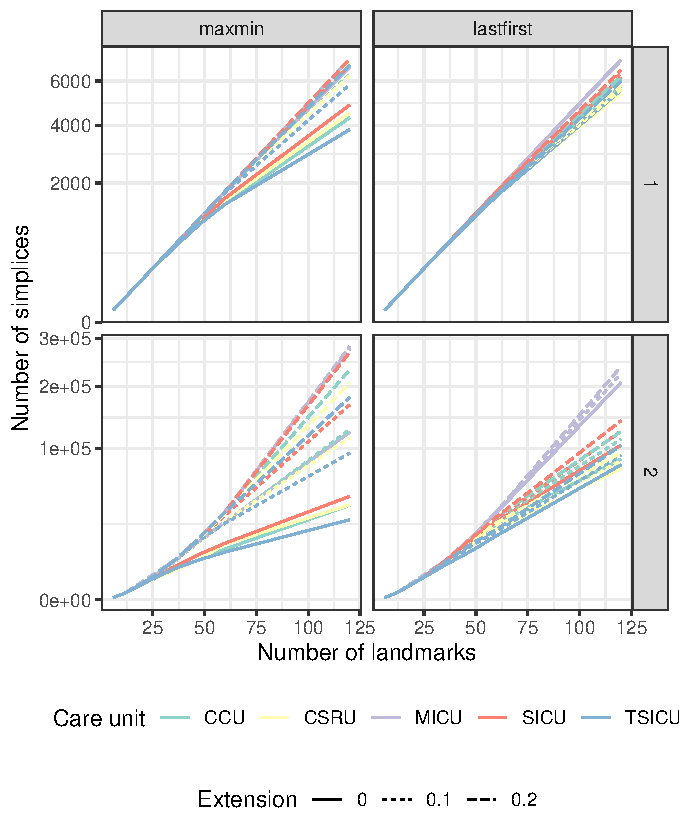
\includegraphics[width=.5\textwidth]{../figures/cover-simplices}
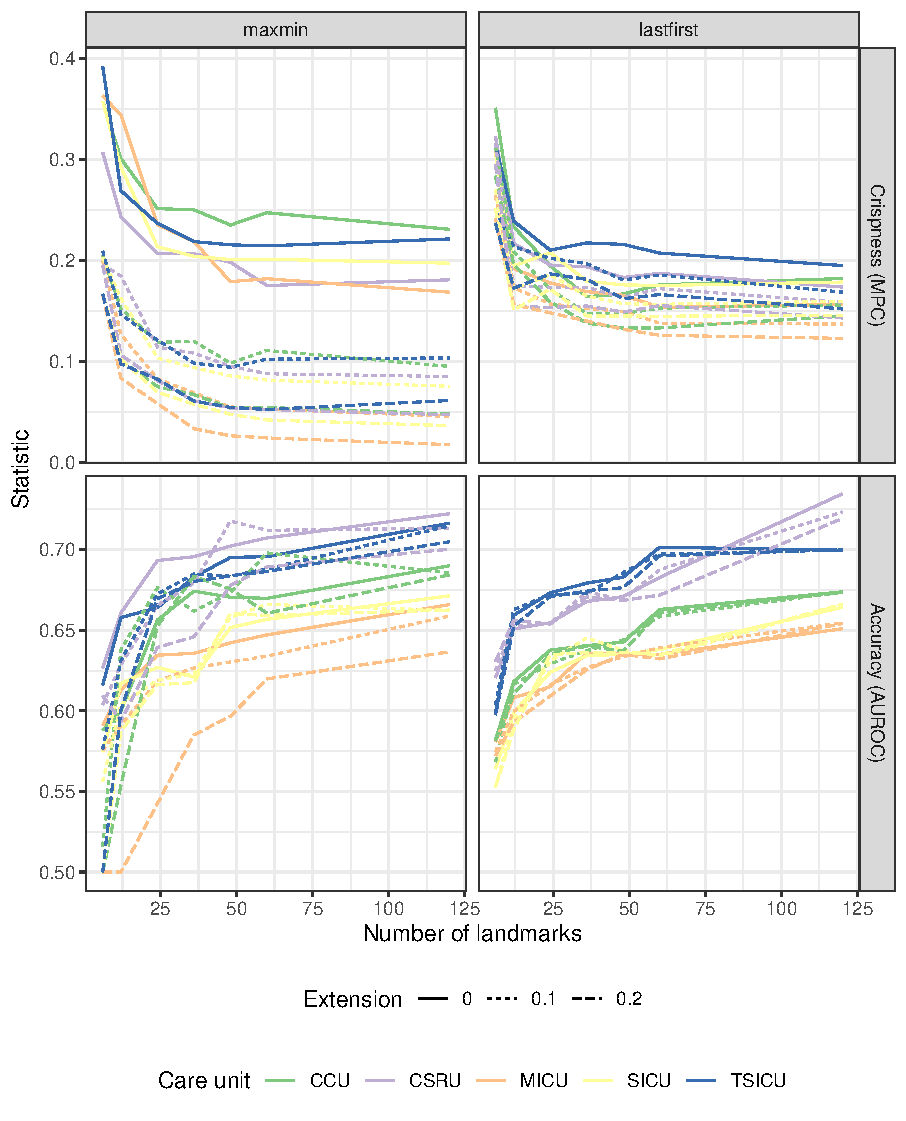
\includegraphics[width=.5\textwidth]{../figures/cover-evaluate}
\caption{
Summary and evaluation statistics versus number of 0-simplices (landmarks) for the covers generated using the maxmin and lastfirst procedures, with three multiplicative extensions in their size.
Left: the sizes of their nerves, as numbers of 1- and 2-simplices, using a square root--transformed vertical scale.
Right: the modified partition coefficient (MPC) and the c-statistic of the risk prediction model based on the cover sets (AUROC).
\label{fig:cover-mimic}
}
\end{figure}

Figure\nbs\ref{fig:cover-mx} presents the same evaluations for covers of
the MXDH data. In contrast to the MIMIC experiments, lastfirst-based
nerves of the MXDH data grew sub-polynomially and were significantly
sparser than maxmin-based nerves. Lastfirst covers tended to be crisper,
especially as the number of landmarks and the extension factors
increased. This indicates that the nearest neighborhoods formed a more
parsimonious cover of the data than the centered balls. The predictive
accuracies of the cover set--based models converged with increasing
numbers of landmarks\footnote{We should increase the maximum number of
  landmarks to be sure.}, though for smaller numbers different selection
procedures performed best for different outcomes.

\begin{figure}
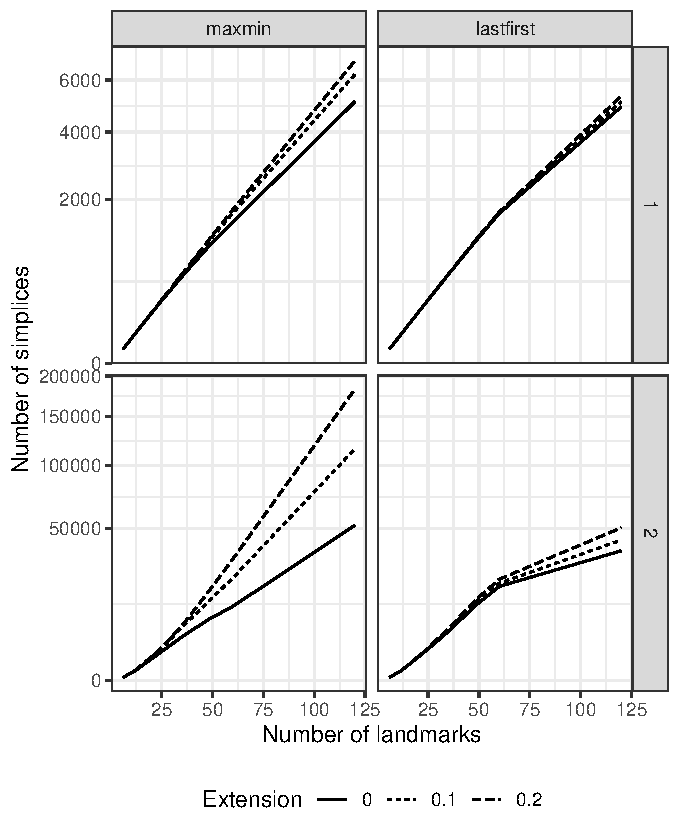
\includegraphics[width=.5\textwidth]{../figures/cover-simplices-mx}
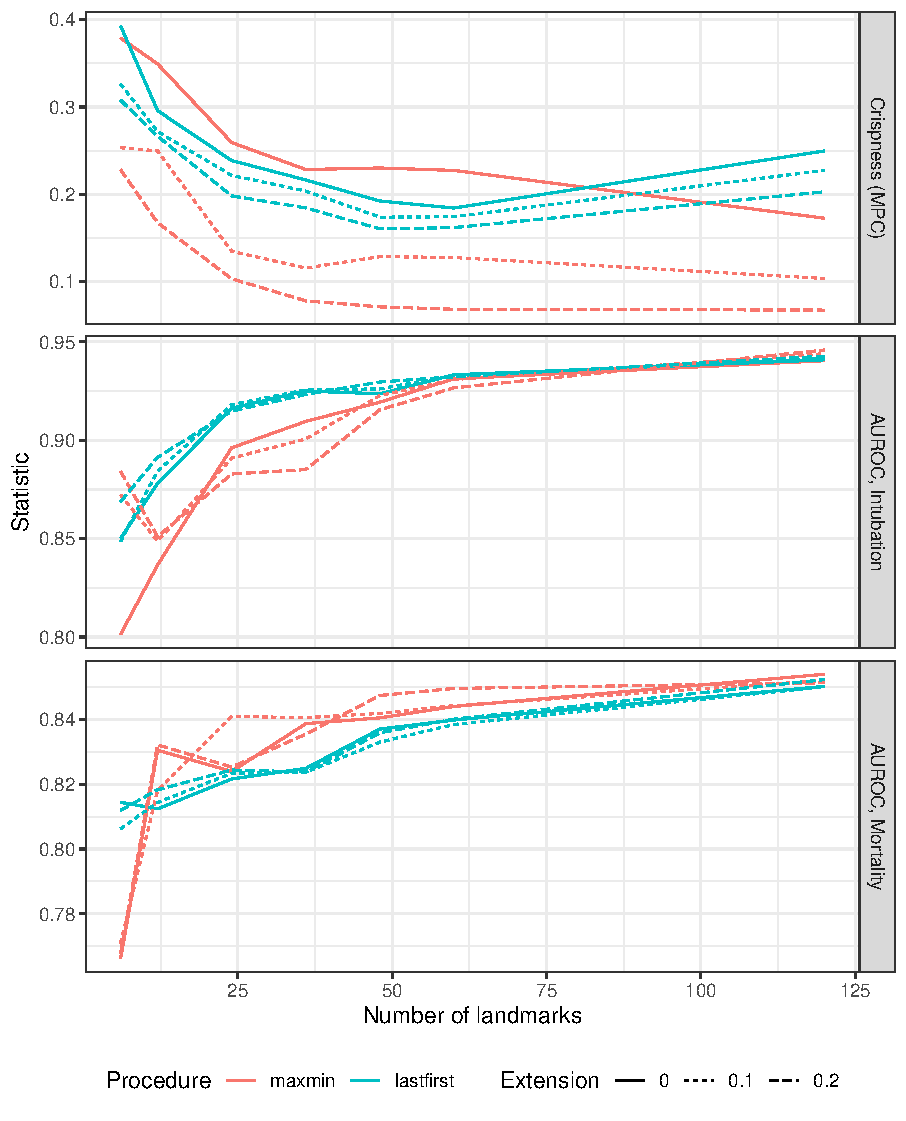
\includegraphics[width=.5\textwidth]{../figures/cover-evaluate-mx}
\caption{
Summary and evaluation statistics versus number of 0-simplices (landmarks) for the covers generated using the maxmin and lastfirst procedures, with three multiplicative extensions in their size.
Left: the sizes of their nerves, as numbers of 1- and 2-simplices, using a square root--transformed vertical scale.
Right: the modified partition coefficient (MPC) and the c-statistics of the risk prediction models based on the cover sets (AUROC).
\label{fig:cover-mx}
}
\end{figure}

\hypertarget{interpolative-nearest-neighbors-prediction}{%
\subsection{Interpolative nearest neighbors
prediction}\label{interpolative-nearest-neighbors-prediction}}

Landmark points may also be used to trade accuracy for memory in
neighborhood-based prediction modeling. Consider the following approach:
A modeling process involves predictor data \(X \in \R^{n \times p}\) and
response data \(y \in \R^{n \times 1}\), partitioned into training and
testing sets \(X_0,X_1\) and \(y_0,y_1\) according to a partition
\(I_0 \sqcup I_1 = \{1,\ldots,n\}\) of the index set. Given
\(x \in X_1\), a nearest neighbors model computes the prediction
\(p(x) = \frac{1}{k}\sum_{q(x,x_i) \leq k}{y_i}\) by averaging the
responses for the \(k^\text{th}\) nearest neighbors of \(x\) in \(X_0\).
By selecting a landmark set \(L \subset X_0\), a researcher can reduce
the computational cost of the model as follows: For each \(\ell \in L\),
calculate \(p(\ell)\) as above. Then, for each \(x \in X_1\), calculate
\(p_L(x) = \sum_{\ell \in L}{w(d(x,\ell)) p(\ell)} / \sum_{\ell \in L}{w(d(x,\ell))}\),
where \(w : \R_{\geq 0} \to \R_{\geq 0}\) is a weighting function (for
example, \(w(d)=d^{-1}\)). The nearest neighbor predictions for \(L\)
thus serve as proxies for the responses associated with \(X_0\).

We took this approach to the prediction of in-hospital mortality for
patients with records in each critical care unit of MIMIC-III. We then
implemented the following procedure:

\begin{enumerate}
\def\labelenumi{\arabic{enumi}.}
\tightlist
\item
  Determine a nested \(6 \times 6\)--fold split for train--fit--test
  cross-validation. That is, partition
  \([n] = \bigsqcup_{i=1}^{6}{I_i}\) into roughly equal parts, and
  partition each \([n] \wo \cl{I_i} = \bigsqcup_{j=1}^{6}{J_{ij}}\) into
  roughly equal parts.
\item
  Iterate the following steps over each \(i,j\):

  \begin{enumerate}
  \def\labelenumii{\alph{enumii})}
  \tightlist
  \item
    Generate a sequence \(L\) of landmarks from the points
    \(X_{([n] \wo \cl{I_i}) \wo \cl{J_{ij}}}\).
  \item
    Identify the \(180\) nearest neighbors \(N^+_{180}(\ell)\) of each
    landmark \(\ell\). This was a fixed parameter, chosen for being
    slightly larger than the optimal neighborhood size in a previous
    study of individualized models {[}@Lee2015{]}.
  \item
    Find the value of \(k \in [180]\) and the weighting function \(w\)
    (among those available) for which the predictions
    \(p_L : X_{J_{ij}} \to [0,1]\) maximize the AUROC.
  \item
    Use the AUROC to evaluate the performance of the predictions
    \(p_L : X_{I_i} \to [0,1]\) using these \(k\) and \(w\).
  \end{enumerate}
\end{enumerate}

We replicated the experiment for each combination of procedure (random,
maxmin, lastfirst) and number of landmarks (\(\abs{L}=36,60,180,360\)).
We hypothesized that, as measured by overall accuracy of the resulting
predictive model, the maxmin and lastfirst procedures would outperform
random selection, and that lastfirst would outperform maxmin, for
similar reasons to those in the previous section.

Boxplots of the AUROCs for each cross-validation step are presented in
Figure\nbs\ref{fig:knn-mimic}. While both landmark procedures yielded
stronger results than random selection, lastfirst performed on average
slightly worse than maxmin on each data set. Importantly, both landmark
procedures also yielded more accurate predictions than a basic
unweighted nearest-neighbors model, lending support to the modeling
approach itself. Interestingly, only on the largest data set (the MICU)
did increasing the number of landmarks from 36 to 360 appreciably
improve predictive accuracy (using all three selection procedures).

\begin{figure}
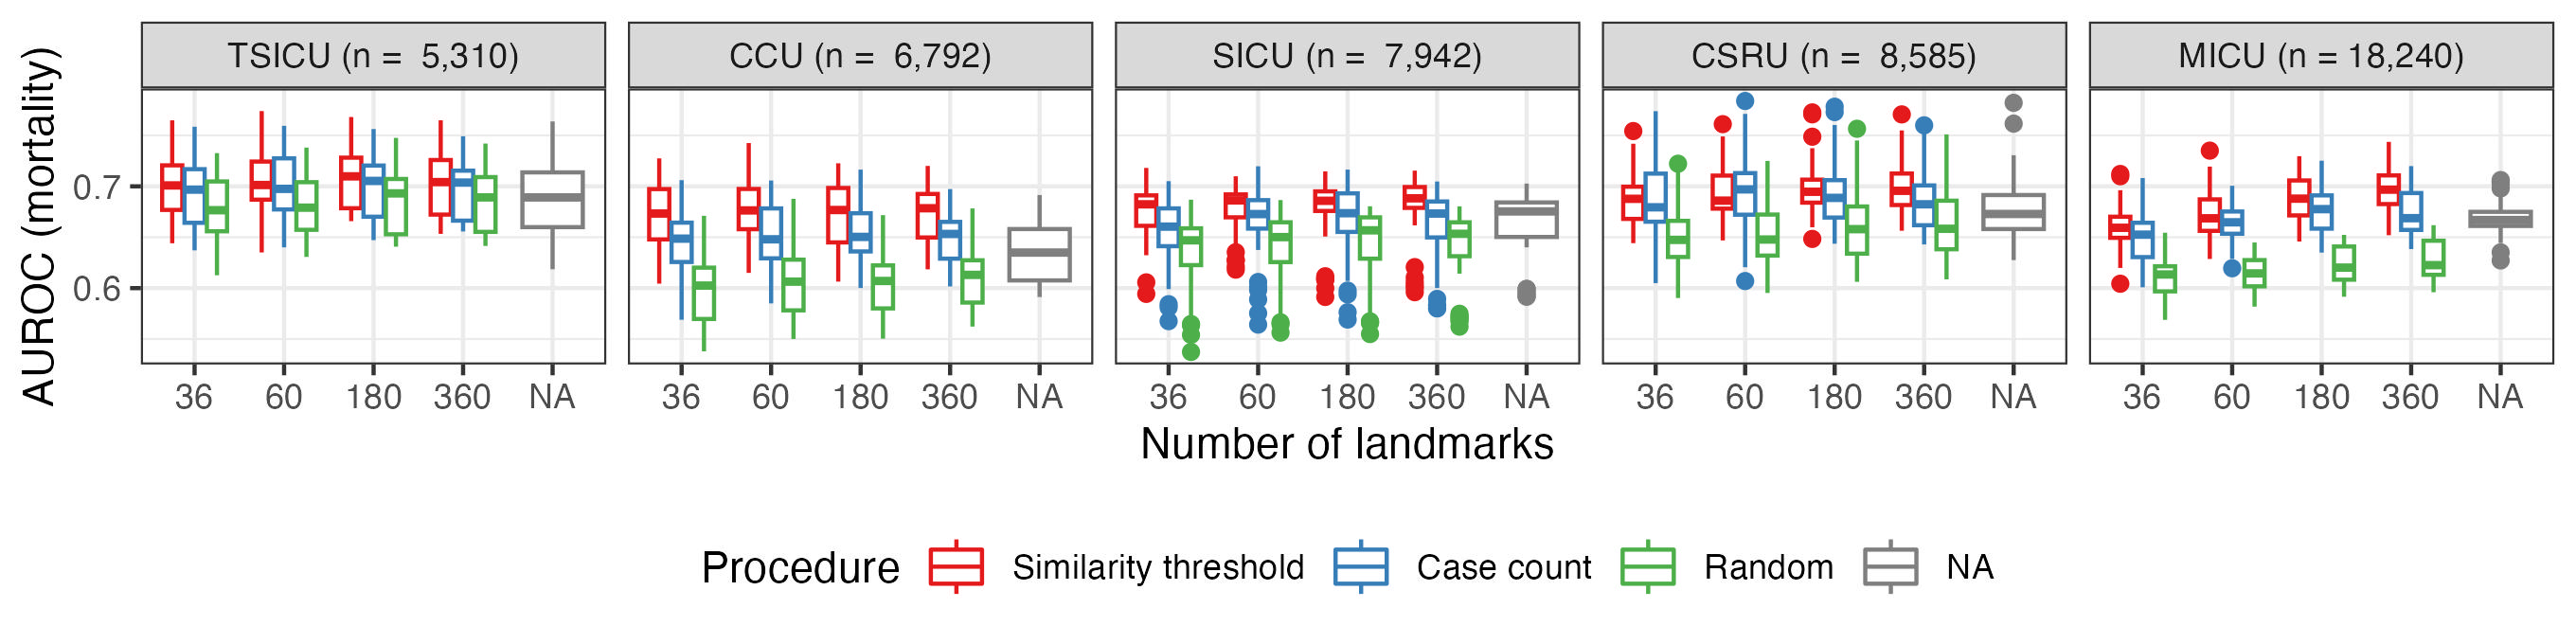
\includegraphics[width=\textwidth]{../figures/knn-auc}
\caption{
AUROCs of the interpolative predictive models of mortality in five MIMIC-III care units based on covers constructed using random, maxmin, and lastfirst procedures to generate landmarks.
Each boxplot summarizes AUROCs from $6 \times 6 = 36$ models, one for each combination of outer and inner fold.
AUROCs of simple nearest-neighbor predictive models are included for comparison.
\label{fig:knn-mimic}
}
\end{figure}

Over the course of the COVID-19 pandemic, hospitals and other facilities
experienced periods of overburden and resource depletion, and best
practices were continually learned and disseminated. As a result,
outcomes in the MXDH data reflect institutional- as well as
population-level factors. We took advantage of the rapid learning
process in particular by adapting the nested CV approach above to a
nested-longitudinal CV approach: We partitioned the data by week,
beginning with Week\nbs11 (March\nbs11--17) and ending with Week\nbs19
(May\nbs6--9, the last dates for which data were available). For each
week \(i\), \(11 < i \leq 19\), we trained prediction models on the data
from Week \(i-1\). We then randomly partitioned Week\nbs\(i\) into six
roughly equal parts and optimized and evaluated the models as above.
(For this analysis, we only considered Gaussian weighting.)

Line plots of model performance are presented in
Figure\nbs\ref{fig:knn-mx}, with one curve (across numbers of landmarks)
per selection procedure, outcome, and week. Again both landmark
selection procedures yielded stronger results than random selection.
Interestingly, this was more pronounced in later weeks, as the pandemic
progressed, even as overall predictive accuracy declined.\footnote{Do we
  know what major events in Brazil might have influenced these outcomes?
  We should at least also plot the number of cases, stratified by
  outcomes, per day over this period.} Overall, performance improved
slightly as the number of landmarks increased from 50 to 150 but either
plateaued or declined from 150 to 250.

\begin{figure}
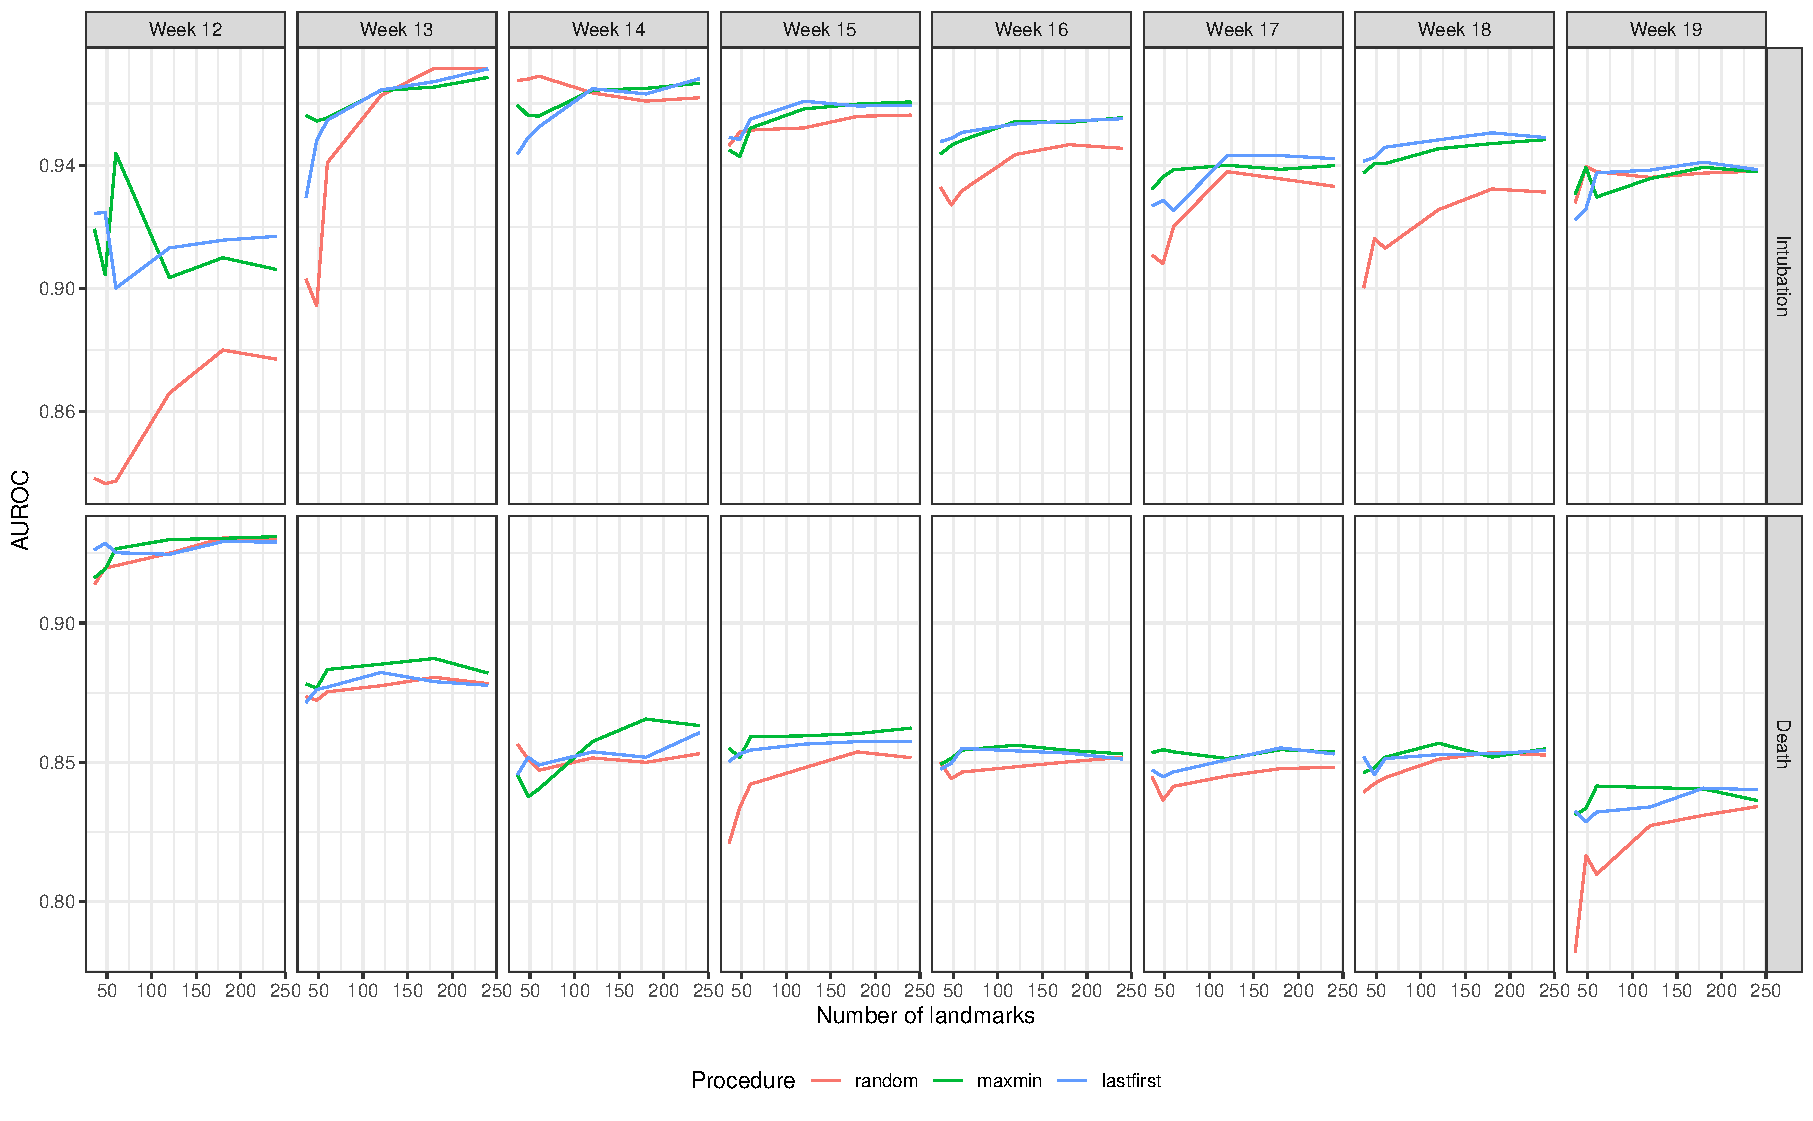
\includegraphics[width=\textwidth]{../figures/knn-auc-mx-gaussian}
\caption{
AUROCs of the sliding-window interpolative predictive models of intubation and mortality in the MXDH data based on covers constructed using random, maxmin, and lastfirst procedures to generate landmarks.
\label{fig:knn-mx}
}
\end{figure}

\hypertarget{discussion}{%
\section{Discussion}\label{discussion}}

The definitions of our lastfirst and firstlast procedures are analogous
to those of maxmin and minmax, substituting ranks in the role of
distances. In this way, lastfirst is an alternative to maxmin that is
adaptive to the local density of the data, similar to the use of fixed
quantiles in place of fixed-length intervals. The maxmin and lastfirst
procedures implicitly construct a minimal cover whose sets are centered
at the selected landmarks, and the fixed-radius balls of maxmin
correspond to the fixed-cardinality neighborhoods of lastfirst. The
rank-based procedures are more combinatorially complex and
computationally expensive, primarily because relative ranks are
asymmetric, which doubles (in the best case) or squares (in the worst
case) the number of distances that must be calculated. Nevertheless, the
procedure can be performed in a reasonable time for many real-world
uses.

We ran an experiment to compare maxmin and lastfirst landmarks at
expediting the computation of persistent homology, extending an
experiment of @deSilva2004. In addition to a uniform sample from a
sphere, we drew skewed and bootstrapped samples in order to simulate
data sets with variable density and multiplicity, in this case
exhibiting a statistical void at one pole of the sphere, opposite a
concentration at the other pole. Whereas the maxmin procedure would
sample more uniformly across the sphere despite this skew, the lastfirst
procedure would concentrate landmarks toward the south. Classical
persistent homology is notoriously sensitive to outliers, and maxmin
better recovered spherical homology than lastfirst, as expected. This is
likely due in part to the filtration itself being based on distances
rather than relative ranks between landmarks (and other points as
witnesses). Yet, compared to random sampling, lastfirst still
oversampled from less dense regions. This is desirable for settings,
such as healthcare, in which regions of missingness often indicate
limitations of the data collection rather than rarity of case types in
the population.

We also ran several experiments that used landmarks to obtain
well-separated clusters of patients with common risk profiles and to
more efficiently generate nearest neighbor predictions. Because we
designed lastfirst to produce cover sets of equal size despite variation
in the density or multiplicity of the data, we expected it to outperform
maxmin with respect to the crispness of clusters and to the accuracy of
predictions. In particular, we expected that the optimal neighborhood
size for outcome prediction would be roughly equal across our data; as a
result, by assigning each landmark case an equally-sized cohort of
similar cases, we expected predictions based on these cohorts to
outperform those based on cohorts using a fixed similarity threshold.

Contrary to expectations, maxmin produced crisper clusterings on
average, and in the case of MIMIC-III more accurate predictions.
However, when the sets of these covers had their radii or cardinalities
extended by a fixed proportion, those of lastfirst better preserved
these qualities. Additionally, in the case of MXDH, neither landmark
selection procedure produced consistently more accurate predictions.

A possible explanation for the stronger performance of maxmin on MIMIC
is that the data did not exhibit very strongly the patterns for which
the lastfirst procedure is designed to account, namely variation in
density and multiplicity. As a result, the RT-similarity measure is in
fact meaningful across the population: Whatever the baseline
presentation of a patient, rather than a cohort of similar patients of
some fixed size, their prognosis would be better guided by a cohort cut
off at a fixed minimum similarity (or maximum distance). This suggests
that the use of personalized cohorts to improve predictive modeling, as
employed by @Lee2015, may be strengthened by optimizing a fixed
similarity threshold rather than a fixed cohort size. In contrast, this
stronger performance was not evident on MXDH, which contained fewer
variables and as a result exhibited many more occurrences of
duplication. It is worth noting that @Park2006, to our knowledge the
only other investigators who have compared predictive models based on
cohorts bounded by a radius versus a cardinality, reached a similar
conclusion.

Another way to think about these results is in terms of a balance
between relevance and pwoer, with fixed-radius balls (respectively,
fixed-cardinality neighborhoods) providing training cohorts of roughly
equal relevance (statistical power) to all test cases. With sufficiently
rich data, relevance can be more precisely measured and becomes more
important to cohort definition, as with MIMIC. When variables are fewer,
as with MXDH, relevance is more difficult to measure, so that larger
samples can improve performance even at the expense of such a measure.

\hypertarget{appendix}{%
\section{Appendix}\label{appendix}}

\hypertarget{relative-ranks}{%
\subsection{Relative ranks}\label{relative-ranks}}

This section develops a more general lastfirst procedure and makes
rigorous some ideas in the main text.

Relative ranks are a much more general notion of metric that encompasess
ranks in nearest neighborhoods.

\begin{definition}[relative rank]
    A \emph{relative rank} on $X$ is a binary relation $q: X \times X \to \R_{\geq 0}$ subject only to the following inequality:
    \begin{equation}\label{eqn:relative-rank}
        \forall x,y \in X : d(x,x) \leq d(x,y)
    \end{equation}
\end{definition}

Relative ranks can be used as the basis for a much more general maxmin
procedure, taking care in particular to account for asymmetry.

Given a relative rank \(q\) on \(X\), write \begin{align*}
    q(Y,Z) &= \min_{y\in Y,z\in Z}{q(y,z)} & Q(Y,Z) &= \max_{y\in Y,z\in Z}{q(y,z)} \\
    q(x,Y) &= q(\{x\},Y)                   & Q(x,Y) &= Q(\{x\},Y) \\
    q(Y,x) &= q(Y,\{x\})                   & Q(x,Y) &= Q(Y,\{x\}) \\
\end{align*}

A pseudometric \(d_X\) induces a relative rank that takes values in
\(\N\) given by the ordinal of one point's distance from another:

\begin{definition}[out-rank and in-rank]
    For $x,y\in X$ with pseudometric $d$, define the \emph{out-rank} $q_{X,d} : X \times X \longrightarrow \N$ as follows:
    \begin{equation}\label{eqn:out-rank}
        q_{X,d}(x,y)=\abs{\{z\in X \mid d(x,z) < d(x,y)\}}%>
    \end{equation}
    and the \emph{in-rank} $q_{X,d}^\top(x,y) = q_{X,d}(y,x)$.
\end{definition}

As with \(d\), we allow ourselves to write \(q=q_{X,d}\) when clear from
context. Note that \(q_{X,d}\) is a relative rank with \(q(x,x)=0\),
\(q(x,y) < N\), and \(\forall x,y \in X : q(x,x) \leq q(x,y)\).

\begin{example}\label{ex:relative-rank}
    Recall $X=\{a,b,c,d\}$ from Example\nbs\ref{ex:relative-rank-max}.
    Lack of symmetry of $q$ is shown by points $b$ and $c$ :
    \begin{align*}
        q(a,c) &= \abs{\{x \in X \mid \abs{x-a} < \abs{c-a} = 2\}} &
        q(c,a) &= \abs{\{x \in X \mid \abs{x-c} < \abs{a-c} = 2\}} \\
               &= \abs{\{a, b\}} &&= \abs{\{b, c, d\}} \\
               &= 2 &&= 3
    \end{align*}

    Observe in particular that $\max_{x\in X}{q(a,x)}=2<\abs{X}-1$; $q(x,\,\cdot\,)$ will not max out at $N-1$ when the most distant points from $x$ have multiplicity.

    However, $q(x,x) = 0$ whether $x$ has multiplicity or not:
    \begin{align*}
        q(a,a) &= \abs{\{x \in X \mid \abs{x-a} < \abs{a-a} = 0\}} &
        q(c,c) &= \abs{\{x \in X \mid \abs{x-c} < \abs{c-c} = 0\}} \\
               &= \abs{\varnothing} &&= \abs{\varnothing} \\
               &= 0 &&= 0
    \end{align*}
\end{example}

We also term the unary rankings \(q(x,\,\cdot\,)\) and
\(q(\,\cdot\,,x)\) the \emph{out- (from $x$)} and
\emph{in- (to $x$) rankings} of \(X\), respectively. These can be used
to define \emph{out-} and \emph{in-neighborhoods} of \(x\).\footnote{The
  terminology and notation are adapted from graph theory. These
  definitions are the same as those for a complete directed graph on
  \(X\) with directed arcs \(x\to y\) weighted by \(q(x,y)\).}

A relative rank \(q\) can be used to define \(k\)-neighborhoods in
greater generality:

\begin{definition}[$k$-neighborhoods using relative rank]
    For $x \in X$, define the \emph{$k$-out-neighborhoods} $N^+_k$ and \emph{$k$-in-neighborhoods} $N^-_k$ of $x$ as the sets
    \begin{align*}
        & N^+_k(x)=\{y\in X\mid q(x,y)\leq k\} \\
        & N^-_k(x)=\{y\in X\mid q(y,x)\leq k\}
    \end{align*}
    Given a subset $Y \subseteq X$, we also define
    \begin{align*}
        & N^+_k(x,Y)=\{y\in Y\mid q_X(x,y)\leq k\} \\
        & N^-_k(x,Y)=\{y\in Y\mid q_X(y,x)\leq k\}
    \end{align*}
\end{definition}

Relative ranks are not as straightforward to compare among subsets of
points. For example, for \(y\neq x\), \(q(x,y)\) takes integer values
between \(\abs{\supp{\{x\}}}\) and \(N-1\). However, they do provide us
with a definition of the lastfirst procedure that straightforwardly
adapts Definition\nbs\ref{def:maxmin}.

\begin{lemma}[firstlast and lastfirst using relative rank]
    Given $Y\subset X$ and a pseudometric $d$ on $X$ with relative rank $q$,
    \begin{align*}
        \lf(Y;X,d) &= \maxmin(Y;X,q_d) \\
        \lf(X,d) &= \maxmin(X,q_d)
    \end{align*}
\end{lemma}

\begin{proof}
This follows directly from the observations
\begin{align*}
    \maxmin(Y;X,q) &= \{x\in X\wo \cl{Y}\mid N_\bullet^-(x,Y) = \max_{y\in X\wo \cl{Y}}{N_\bullet^-(y,Y)}\} \\
    \maxmin(X,q) &= \{x\in X\mid N_\bullet^-(x,X \wo \cl{\{x\}}) = \max_{y\in X}{N_\bullet^-(y,X \wo \cl{\{y\}}}\}
\end{align*}
obtained by adapting Proposition\nbs\ref{prop:maxmin} to the relative rank.
\end{proof}

\hypertarget{selection-procedures}{%
\subsubsection{Selection procedures}\label{selection-procedures}}

The choice of \(\ell_i \in \maxmin(L)\) is trivial when \(X\) is in
locally general position, but this study is specifically interested in
cases with a high frequency of violations of this property, and indeed
with such violations of Hausdorffness that large numbers of points in
\(X\) may be co-located. When \(X\) is not in locally general position,
the choice of selection from among the maxmin set is consequential. For
convenience, let \(\maxmin(L;X)\) take the value \(\varnothing\) if
\(\cl{L}=X\) and the value \(X\) if \(L=\varnothing\). Then write
\(\graph{\maxmin, X} \subset \order{X} \times \power{X}\) for the graph
of the unary function \(\maxmin(\,\cdot\,;X): \order{X} \to \power{X}\),
so that \((L,\Gamma) \in \graph{\maxmin, X}\) if and only if
\(\maxmin(L;X) = \Gamma\). Then a selection procedure is a function
\(\sigma: \graph{\maxmin, X} \to X\) subject to
\(\sigma((L,\Gamma)) \in \Gamma = \maxmin(L;X)\). Importantly,
\(\sigma\) may depend not only on the maxmin set \(\Gamma\) but also on
the ordered sequence \(L\).

We assume the following choice of \(\sigma\): Take
\(d_L = \max_{y \in X \wo \cl{L}}{d(y,L)}\). For each
\(y \in \maxmin(L;X)\), choose \(\ell_y \in L\) for which
\(d(y,\ell_y) = d_L\). Then take
\(\maxmin^{(1)}(L;X) = \{y \in \maxmin(L;X) \mid d(y,L \wo \{\ell_y\}) = \max_{z \in \maxmin(L;X)}{d(z,L \wo \{\ell_z\})}\}\).
While \(\abs{\maxmin^{(j)}(L;X)} > 1\), continue in this way until
either a singleton is reached or \(j=\abs{L}=i\). If the latter, then
the choice \(\sigma\) is arbitrary among the remaining \(y\).\footnote{Should
  this be written up as an algorithm?}

\hypertarget{algorithms}{%
\subsubsection{Algorithms}\label{algorithms}}

Algorithm\nbs\ref{alg:lastfirst-landmarks} calculates a lastfirst set
from a seed point, subject to parameters analogous to \(n\) and
\(\epsilon\) in Algorithm\nbs\ref{alg:maxmin}. The algorithm is tailored
to the vectorized arithmetic of R, and Lemma\nbs\ref{lem:revlex-lex}
provides a shortcut between \(Q^-\) and the more compact way that the
relative rank data are stored.

\begin{lemma}\label{lem:revlex-lex}
For $L = \{ \ell_0, \ldots, \ell_n \} \subset X$, write $S(x,L) = ( q(\ell_{\pi^{-1}(1)},x) \leq \cdots \leq q(\ell_{\pi^{-1}(n)},x) )$, where $\pi$ is any suitable permutation on $[n]$.
Then $Q^-(x,L) < Q^-(y,L) \Leftrightarrow S(x,L) < S(y,L)$.
\end{lemma}

\begin{proof}
Write $Q(x) = Q^-(x,L)$ and $Q(y) = Q^-(y,L)$ and suppose that $Q(x) < Q(y)$.
This means that $Q_i(x) > Q_i(y)$ for some index $i \in [N]$ while $Q_j(x) = Q_j(y)$ for all $j < i$.
There are then, for each $j < i$, equal numbers of $\ell \in L$ for which $q(\ell,x) = j$ and for which $q(\ell,y) = j$; while there are more $\ell \in L$ for which $q(\ell,x) = i$ than for which $q(\ell,y) = i$.
When the sets $\{ q(\ell,x) \}_{\ell in L}$ and $\{ q(\ell,y) \}_{\ell in L}$ are arranged in order to get $S(x,L)$ and $S(y,L)$, therefore, the leftmost position at which they differ is $Q_1(y) + \cdots + Q_i(Y) + 1$, at which $q(\ell,x) = i$ while $q(\ell,y) \geq i + 1$.
Thus $S(x,L) <_{\operatorname{lex}} S(y,L)$.

The reverse implication is similarly straightforward.
\end{proof}

\begin{algorithm}
\caption{Calculate the lastfirst landmark sequence from a seed point.}
\label{alg:lastfirst-landmarks}
\begin{algorithmic}[1]
\REQUIRE finite pseudometric space $(X,d)$
\REQUIRE seed point $\ell_0 \in X$
\REQUIRE number of landmarks $n \in \N$ or cover set cardinality $k \in \N$
\REQUIRE selection procedure $\sigma$
\STATE if $n$ is not given, set $n \leftarrow 0$
\label{line:n}
\STATE if $k$ is not given, set $k \leftarrow \infty$
\label{line:k}
\STATE $L \leftarrow \varnothing$ initial landmark set
\STATE $F \leftarrow \{ \ell_0 \}$ initial lastfirst set
\STATE $R \in \N^{N \times 0}$, a $0$-dimensional $\N$-valued matrix
\FOR{$i$ from $0$ to $\uniq{X} - 1$}
    \STATE $\ell_i \leftarrow \sigma(F)$
    \STATE $L \leftarrow L \cup \{\ell_i\}$
    \STATE $D_i \leftarrow (d_{i1},\ldots,d_{iN}) \in {\R_{\geq 0}}^N$, where $d_{ir} = d(\ell_i, x_r)$
    \STATE $Q_i \leftarrow \verb|rank|(D_i) \in {\N_{\geq 0}}^N$ (so that $Q = (q(\ell_i, x_1),\ldots,q(\ell_i, x_N))$)
    \label{line:rank}
    \STATE $R \leftarrow [R, Q_i] \in \N^{N \times (i+1)}$
    \STATE $k_{\min} \leftarrow \max_{r=1}^{N}{ \min_{j=1,i+1}{ R_{r,j} } }$ (minimum $k$ for which neighborhoods centered at $L$ cover $X$)
    \label{line:kmin}
    \IF{$D(L, X \wo \cl{L}) = 0$}
        \STATE \textbf{break}
        \label{line:nonempty}
    \ENDIF
    \IF{$i \geq n$ and $k_{\min} \leq k$}
        \STATE \textbf{break}
        \label{line:check}
    \ENDIF
    \STATE $R \leftarrow [ \verb|sort|({R_{1,\bullet}})^\top \cdots \verb|sort|({R_{N,\bullet}})^\top ]^\top \in \N^{N \times (i+1)}$
    \label{line:sort}
    \STATE $F \leftarrow X \wo \cl{L}$
    \FOR{$j$ from $1$ to $i$}
    \label{line:maximize}
        \STATE $F \leftarrow \{x_r \in F \mid R_{rj} = \max_{r'}{R_{r'j}}\}$
        \label{line:lastfirst}
        \IF{$\abs{F} = 1$}
            \STATE \textbf{break}
        \ENDIF
    \ENDFOR
\ENDFOR
\RETURN $L$
\RETURN lastfirst landmark set $L$ with at least $n$ cover sets of cardinality at most $k$
\end{algorithmic}
\end{algorithm}

\begin{proposition}
Algorithm\nbs\ref{alg:lastfirst-landmarks} returns a lastfirst landmark set.
If $n \leq \uniq{X}$ is given as input and $k$ is not, then $\abs{L} = n$.
If $n$ and $k$ are both given, then $\abs{L} \geq n$.
Otherwise, $L$ is minimal in the sense that no proper prefix of $L$ gives a cover of $X$ by $k$-nearest neighborhoods.
\end{proposition}

\begin{proof}
Let $(X,d)$ be a finite metric space and $\ell_0 \in X$ be a seed point, as required by Algorithm\nbs\ref{alg:lastfirst-landmarks}.
Note that, for the algorithm to terminate its loop and subsequently return $L$, either there must be no points in $X \wo \cl{L}$ distinguishable from $L$ (line\nbs\ref{line:nonempty}), or both of two exit conditions must hold (line\nbs\ref{line:check}):
  (1) $k_{\min} \leq k$ and
  (2) $\abs{L} \geq n$.

Because the seed point is arbitrary, for the main result it is enough to show that, at each step $i$, $F = \lf(\{ \ell_0, \ldots, \ell_{i-1} \})$.
When $F$ is calculated on line\nbs\ref{line:lastfirst}, the rows $R_r$ of $R$ contain the in-ranks $q(\ell_i, x_r)$ of $x_r$ in increasing order.
Because $D(L, X \wo \cl{L}) > 0$ (line\nbs\ref{line:nonempty}), $F$ is nonempty.
By Lemma\nbs\ref{lem:revlex-lex}, then, $Q^-(x_r, L)$ is maximized (in revlex) when $R_r$ is maximized in lex, and this is exactly what the loop that begins on line\nbs\ref{line:maximize} does.

Suppose first that $n \leq \uniq{X}$ is given.
The loop will only break on line\nbs\ref{line:nonempty} if $D(L, X \wo \cl{L}) = 0$, which is only possible if $\abs{L} = \uniq{X} \geq n$.
The loop will only break on line\nbs\ref{line:check} if both $\abs{L} = i \geq n$ and $k_{\min} \leq k$.
Since these are the only two possible breaks, $\abs{L} \geq n$ is a necessary condition.
\footnote{Note that $\abs{L} > n$ if and only if $k_{\min} \leq k$ is not satisfied when $\abs{L} = n$, meaning that $X$ would not be covered by $k$-neighborhoods around $n$ landmark points, so that more landmarks must be chosen to guarantee the algorithm produces a valid $k$-neighborhood cover.}

If $k$ is not given, then $k$ is set to $\infty$ on line\nbs\ref{line:k}, which means that (1) holds throughout the loop.
Then the algorithm terminates as least as soon as (2) is satisfied, when $\abs{L} = n$, and as discussed above it cannot terminate any sooner.

Now suppose $n$ is not given.
Then $k$ must be given, and $n$ is set to $0$ (line\nbs\ref{line:n}).
This means that (2) always holds, so the algorithm terminates as soon as (1) is satisfied, i.e.\ when $k \geq k_{\min}$ with $k_{\min}$ as defined on line\nbs\ref{line:kmin}.
We claim that
\[ k_{\min} = \max_{x \in X}{ \min_{\ell \in L}{ q(\ell, x) } } \]
which means that every point in $x$ is within a $k$-neighborhood of some existing landmark $\ell \in L$, i.e.\ that the $k$-neighborhoods at $L$ constitute a cover of $X$.
For this to have not been true for $L$ at previous iterations, there must have been $x \in X$ with $q(\ell, x) > k$ for all $\ell \in L$, meaning that the $k$-neighborhoods at $L$ did not cover $X$.

To prove the claim, note that the maximum is taken over all rows of $R$, which at no point in the algorithm are permuted---that is, the entries of row $R_{r,\bullet}$ at each iteration consist of $q(\ell_0,x_r),\ldots,q(\ell_i,x_r)$ in some order.
Therefore, $\min_{j=1}^{i}{R_{r,j}} = \min_{\ell \in L}{ q(\ell, x_r) }$.
Because columns $1$ through $i-1$ of $R$ were sorted in the previous iteration (line\nbs\ref{line:sort}), this minimum only needs to be taken over $j=1,i$, which gives the formula on line\nbs\ref{line:kmin}.
\end{proof}

\hypertarget{tie-handling}{%
\subsubsection{Tie handling}\label{tie-handling}}

We might have defined two relative ranks
\(\check{q}, \hat{q} : X \times X \longrightarrow \N\) (``\(q\)-check''
and ``\(q\)-hat'') as follows: \begin{align*}
& \check{q}(x,y)=\abs{\{z\in X\mid d(x,z)<d(x,y)\}} \\%>
& \hat{q}(x,y)=\abs{\{z\in X\mid d(x,z)\leq d(x,y)\}} - 1
\end{align*} In this notation, \(\check{q}=q\), while \(\hat{q}(x,y)\)
is the cardinality of the smallest ball centered at \(x\) that contains
\(y\). Then
\(\check{N}^\pm_1(x) \subseteq \{x\} \subseteq \hat{N}^\pm_1(x)\), and
\(\hat{q}(x,x)>0\) when \(x\) has multiplicity. The two relative ranks
derive from two tie-handling schemes for calculating rankings of lists
with duplicates. For example, if \(a<b=c<d\) are the distances from
\(x\) to \(y_1,y_2,y_3,y_4\), respectively, then
\((\check{q}(x,y_1),\check{q}(x,y_2),\check{q}(x,y_3),\check{q}(x,y_4))=(0,1,1,3)\)
and
\((\hat{q}(x,y_1),\hat{q}(x,y_2),\hat{q}(x,y_3),\hat{q}(x,y_4))=(0,2,2,3)\).
Indeed, any tie-handling rule could be used, and the choice becomes more
consequential with greater multiplicity in the data.

Conceptually, the lastfirst procedure based on \(\hat{q}\) would produce
landmark sets that yield neighborhood covers with smaller, rather than
larger, neighborhoods in regions of high multiplicity. While we do not
use these ideas in this study, they may be suitable in some settings or
for some purposes, for example when high multiplicity indicates a
failure to discriminate between important categories. It is also
possible that \(\check{q}\)- and \(\hat{q}\)-based covers could be used
to produce interveaving sequences of nerves useful for stability
analysis.

\begin{example}\label{ex:relative-rank-max}
Consider the simple case $X = \{a, b, c, d\}$, visualized below, equipped with the standard Euclidean metric:
\begin{centeredTikz}
    [every label/.append style={text=black!60!blue, font=\scriptsize}]
    \draw[gray] (0,0) -- (5,0);

    \foreach \i in {0,...,3}
        \draw[gray] (\i,0.1) -- + (0,-0.25) node[font=\scriptsize, text=gray, below] {$\i$};
    \draw[gray] (3,0.1) -- + (0,-0.25) node[font=\scriptsize, text=gray, below] {};
    \draw[gray] (5,0.1) -- + (0,-0.25) node[font=\scriptsize, text=gray, below] {$5$};

    \node[circle, draw=blue!60, fill=blue!5, inner sep=0.5mm, label=above:{$a = 1$}] at (1,0) {};
    \node[circle, draw=blue!60, fill=blue!5, inner sep=0.5mm, label=above:{$b = 2$}] at (2,0) {};
    \node[circle, draw=blue!60, fill=blue!5, inner sep=0.5mm, label=above:{$c = 4$}] at (4,0.1) {};
    \node[circle, draw=blue!60, fill=blue!5, inner sep=0.5mm, label=below:{$d = 4$}] at (4,-0.1) {};
\end{centeredTikz}

The relative rank $\hat{q}$ is also asymmetric:
\begin{align*}
    \hat{q}(b,c) &= \abs{\{x \in X \mid \abs{x-b} \leq \abs{c-b} = 2\}} &
    \hat{q}(c,b) &= \abs{\{x \in X \mid \abs{x-c} \leq \abs{b-c} = 2\}} \\
        &= \abs{\{a, b, c, d\}} &&= \abs{\{b, c, d\}} \\
        &= 4 &&= 3
\end{align*}

Observe that $\hat{q}(x,x) = 1$ only for distinguishable points $x \in X$:
\begin{align*}
    \hat{q}(a,a) &= \abs{\{x \in X \mid \abs{x-a} \leq \abs{a-a} = 0\}} &
    \hat{q}(c,c) &= \abs{\{x \in X \mid \abs{x-c} \leq \abs{c-c} = 0\}} \\
       &= \abs{\{a\}} &&= \abs{\{c, d\}} \\
       &= 1 &&= 2
\end{align*}

Finally, observe that $\hat{q}(x,\,\cdot\,)$ always maxes out at $\abs{X}$: $\hat{q}(a,c) = \hat{q}(b,c) = \hat{q}(c,a) = \hat{q}(d,a) = \abs{X}$.

Continuing on as in Example\nbs\ref{ex:rank-neighborhoods}, we can compute $\hat{N}_2^+$ and $\hat{N}_2^-$ for $b$ and $c$:
\begin{align*}
    \hat{N}_2^+ (b) &= \{x \in X \mid \hat{q}(b,x) \leq 2\} &
    \hat{N}_2^+ (c) &= \{x \in X \mid \hat{q}(c,x) \leq 2\} \\
        &= \{a, b\} &&= \{c, d\} \\
        \\
    \hat{N}_2^- (b) &= \{x \in X \mid \hat{q}(x,b) \leq 2\} &
    \hat{N}_2^- (c) &= \{x \in X \mid \hat{q}(x,c) \leq 2\} \\
        &= \{a, b\} &&= \{c, d\}
\end{align*}

Similarly, we can compute the other $\hat{N}_k^+$ and $\hat{N}_k^-$ for $b$ and $c$:
\begin{align*}
    \hat{Q}^+ (b) &= (\abs{\hat{N}^+_1(b)}, \abs{\hat{N}^+_2(b)}, \abs{\hat{N}^+_3(b)}, \abs{\hat{N}^+_4(b)}) &
    \hat{N}_\bullet^+ (c) &= (\abs{\hat{N}^+_1(c)}, \abs{\hat{N}^+_2(c)}, \abs{\hat{N}^+_3(c)}, \abs{\hat{N}^+_4(c)}) \\
        &= (\abs{\{b\}}, \abs{\{a, b\}}, \abs{\{a, b\}}, \abs{\{a, b, c, d\}}) &
        &= (\abs{\varnothing}, \abs{\{c, d\}}, \abs{\{b, c, d\}}, \abs{\{a, b, c, d\}}) \\
        &= (1, 2, 2, 4) &
        &= (0, 2, 3, 4) \\
        \\
    \hat{N}_\bullet^- (b) &= (\abs{\hat{N}^-_1(b)}, \abs{\hat{N}^-_2(b)}, \abs{\hat{N}^-_3(b)}, \abs{\hat{N}^-_4(b)}) &
    \hat{N}_\bullet^- (c) &= (\abs{\hat{N}^-_1(c)}, \abs{\hat{N}^-_2(c)}, \abs{\hat{N}^-_3(c)}, \abs{\hat{N}^-_4(c)}) \\
        &= (\abs{\{b\}}, \abs{\{a, b\}}, \abs{\{a, b, c, d\}}, \abs{\{a, b, c, d\}}) &
        &= (\abs{\varnothing}, \abs{\{c, d\}}, \abs{\{c, d\}}, \abs{\{a, b, c, d\}}) \\
        &= (1, 2, 4, 4) &&= (0, 2, 2, 4)
\end{align*}
\end{example}

\hypertarget{homology-recovery}{%
\subsection{Homology recovery}\label{homology-recovery}}

We compared the suitability of three landmarking procedures (uniformly
random, maxmin, lastfirst) on datasets with varying density and
duplication patterns by extending an example of @deSilva2004. Each
expriment proceeded as follows: We sampled \(n=540\) points from the
sphere \(\Sph^2\subset\R^3\) and in different experiments selected
\(k=12,36,60\) landmark points. We then used the landmarks to compute PH
and computed the \emph{relative dominance} \((R_1 - R_0) / K_0\) and
\emph{absolute dominance} \((R_1 - R_0) / K_1\) of the last interval
over which all Betti numbers agreed with those of \(\Sph^2\). These
statistics provide an indication of how successfully PH recovered the
homology of the manifold from which the points were sampled.

The points \(x=(r,\theta,\phi)\) were sampled using four procedures:
uniform sampling, skewed sampling, uniform sampling with skewed
boosting, and skewed sampling with skewed boosting. The first procedure
was used by @deSilva2004 and here serves as a baseline. For a sample
\(S\) (with multiplicities) generated from each of the other three
procedures, the expected density
\(\lim_{\eps\to 0}\lim_{n\to\infty}\frac{1}{n}\abs{\{x=(r,\theta,\phi)\in S\mid \alpha-\eps<\phi<\alpha+\eps\}}\)
of points near a given latitude \(\alpha\in[0,\pi]\) is proportional to
the quartic function \(p:[0,1]\to[0,1]\) defined by
\(p(x)=(\frac{\phi}{\pi})^4\).\footnote{Should this be analytically
  shown or confirmed using large samples?} Skewed sampling is performed
via rejection sampling: Points \(x_i=(r_i,\theta_i,\phi_i)\) are sampled
uniformly and rejected at random if a uniform random variable
\(t_i\in[0,1]\) satisfies \((\frac{\phi_i}{\pi})^\alpha<t_i\) until
\(n\) points have been kept {[}@Diaconis2013{]}. Skewed boosting is
performed by first obtaining a (uniform or skewed) sample \(T\) of size
a fraction \(\frac{n}{6}\) of the total, then sampling \(n\) points
(with replacement) from \(T\) using the probability mass function
satisfying \(P(x_i)\propto(\frac{\phi_i}{\pi})^\beta\). When performed
separately, skewed sampling and skewed boosting use \(\alpha=\beta=4\);
when performed in sequence, they use \(\alpha=\beta=2\).

The landmark points were selected in three ways: uniform random
selection (without replacement), the maxmin procedure, and the lastfirst
procedure. We computed PH in Python GUDHI, using three implementations:
Vietoris--Rips (VR) filtrations on the landmarks, alpha complexes on the
landmarks, and witness complexes on the landmarks with the full sample
as witnesses {[}@Maria2021; @Rouvreau2021; @Kachanovich2021{]}.

The skewed data sets are dense at the south pole and sparse at the north
pole. We expect lastfirst to be more sensitive to this variation and
place more landmarks toward the south. As measured by dominance,
therefore, we hypothesized that lastfirst would be competitive with
maxmin when samples are uniform and inferior to maxmin when samples are
skewed. Put differently, we expected lastfirst to better reject the
homology of \(\Sph^2\), i.e.~to detect the statistical void at the north
pole.

Figure\nbs\ref{fig:sphere} compares the relative dominance of the
spherical homology groups in each case. When PH is computed using VR or
alpha complexes, maxmin better recovers the homology of the sphere
except on uniform samples, while lastfirst and random selection better
detect the void. Random selection is usually better than lastfirst
selection at detecting this void when samples are non-uniform, which
indicates that lastfirst selection still oversamples from less dense
regions. Lastfirst and maxmin perform similarly when PH is computed
using witness complexes.

\begin{figure}
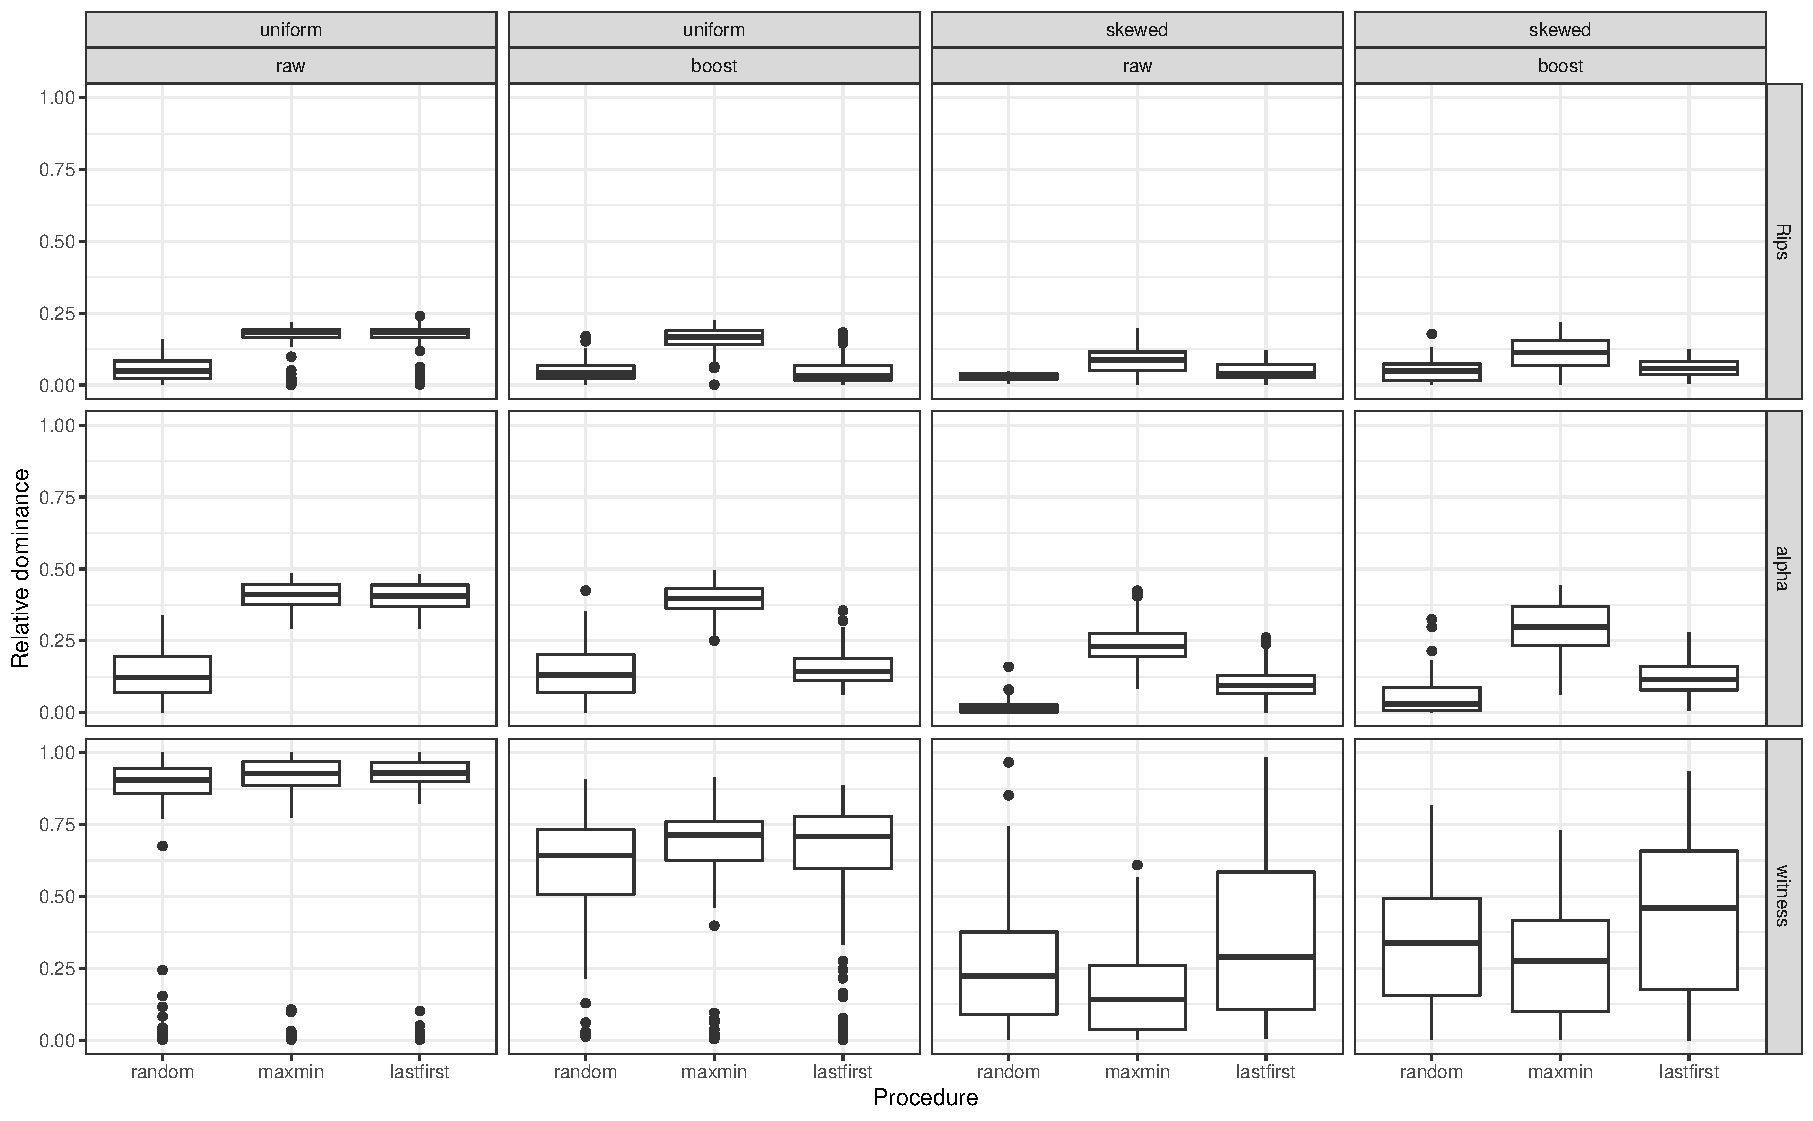
\includegraphics[width=\textwidth]{../figures/homology-sphere-relative}
\caption{
Relative dominance of the spherical homology groups in the persistent homology of four samples from the sphere, using each of three landmark procedures and three persistence computations. Similar plots of absolute dominance (not shown) tell a consistent story, but the distributions are more skewed so the comparisons are less clear.
\label{fig:sphere}
}
\end{figure}

\hypertarget{references}{%
\section{References}\label{references}}

\end{document}
